

%%%%%%%%%%%%%%%%%%%%%%%%%%%%%%%%%%%%%%%%%%%%%%%%%%%%%%%%%%%%%%%%%%%%%%%%%%%%%%%%
%                         FORMATO DE TESIS FI UNAM                             %
%%%%%%%%%%%%%%%%%%%%%%%%%%%%%%%%%%%%%%%%%%%%%%%%%%%%%%%%%%%%%%%%%%%%%%%%%%%%%%%%
% based on Harish Bhanderi's PhD/MPhil template, then Uni Cambridge
% http://www-h.eng.cam.ac.uk/help/tpl/textprocessing/ThesisStyle/
% corrected and extended in 2007 by Jakob Suckale, then MPI-iCBG PhD programme
% and made available through OpenWetWare.org - the free biology wiki

%                     Under GNU License v3

% ADAPTADO PARA FI-UNAM:  @Tepexic
%
\documentclass[twoside,11pt]{Latex/Classes/PhDthesisPSnPDF}
%         PUEDEN INCLUIR EN ESTE ESPACIO LOS PAQUETES EXTRA, O BIEN, EN EL ARCHIVO "PhDthesisPSnPDF.cls" EN "./Latex/Classes/"
%\usepackage[round, sort, numbers]{natbib}  % Personalizar la bibliografía a gusto de cada quien
% Note:
% The \blindtext or \Blindtext commands throughout this template generate dummy text
% to fill the template out. These commands should all be removed when 
% writing thesis content.
\usepackage[letterpaper,lmargin=3cm,rmargin=3cm, top=2.5cm, bottom=4cm ]{geometry}
\usepackage{pdfpages}
\usepackage{verbatim}
\usepackage{fancyvrb}
\usepackage[most]{tcolorbox}
\newtcolorbox{mybox}{colframe=gray!30!gray}
\usepackage{cite}
\usepackage{array}
\usepackage{multirow}
\usepackage{graphicx}
\usepackage{epigraph}
\usepackage{enumerate}
\setlength\epigraphwidth{.8\textwidth}



% This file contains macros that can be called up from connected TeX files
% It helps to summarise repeated code, e.g. figure insertion (see below).

%%%%%%%%%%%%%%%%%%%%%%%%%%%%%%%%%%%%%%%%%%%%%%
%            Colores de la UNAM              %
%%%%%%%%%%%%%%%%%%%%%%%%%%%%%%%%%%%%%%%%%%%%%%
%Azul Pantone 541  -->(0,63,119) RGB
\definecolor{Azul}{RGB}{0,63,119}

%Oro Pantone 460  -->(234,221,150) RGB
\definecolor{Oro}{RGB}{234,221,150}


%%%%%%%%%%%%%%%%%%%%%%%%%%%%%%%%%%%%%%%%%%%%%%
%            Comandos para líneas            %
%%%%%%%%%%%%%%%%%%%%%%%%%%%%%%%%%%%%%%%%%%%%%%
%Se define un comando \colorvrule para hacer líneas verticales de color con 3 argumentos: color, ancho, alto
\newcommand{\colorvrule}[3]{
\begingroup\color{#1}\vrule width#2 height#3
\endgroup}

%Se define un comando \colorhrule para hacer líneas horizontales de color con 2 argumentos: color, ancho
\newcommand{\colorhrule}[2]{
\begingroup\color{#1}\hrule height#2
\endgroup}

%%%%%%%%%%%%%%%%%%%%%%%%%%%%%%%%%%%%%%%%%%%%%%
%          Comando para derivadas            %
%%%%%%%%%%%%%%%%%%%%%%%%%%%%%%%%%%%%%%%%%%%%%%
\newcommand{\derivada}[3][]{\ensuremath{\dfrac{\mbox{d}^{#1}#2}{\mbox{d}#3^{#1}}}} 
%primer argumento(opcional): orden de la derivada
%segundo argumento: función a derivar
%tercer argumento: variable respecto a la que se deriva


%%%%%%%%%%%%%%%%%%%%%%%%%%%%%%%%%%%%%%%%%%%%%%
%       Comando para la exponencial          %
%%%%%%%%%%%%%%%%%%%%%%%%%%%%%%%%%%%%%%%%%%%%%%
\newcommand{\e}[1][]{\ensuremath{\mbox{e}^{#1}}}
%primer argumento(opcional): exponente de la exponencial




% insert a centered figure with caption and description
% parameters 1:filename, 2:title, 3:description and label
\newcommand{\figuremacro}[3]{
	\begin{figure}[htbp]
		\centering
		\includegraphics[width=1\textwidth]{#1}
		\caption[#2]{\textbf{#2} - #3}
		\label{condicion}
	\end{figure}
}

% insert a centered figure with caption and description AND WIDTH
% parameters 1:filename, 2:title, 3:description and label, 4: textwidth
% textwidth 1 means as text, 0.5 means half the width of the text
\newcommand{\figuremacroW}[4]{
	\begin{figure}[htbp]
		\centering
		\includegraphics[width=#4\textwidth]{#1}
		\caption[#2]{\textbf{#2} - #3}
		\label{#1}
	\end{figure}
}

% inserts a figure with wrapped around text; only suitable for NARROW figs
% o is for outside on a double paged document; others: l, r, i(inside)
% text and figure will each be half of the document width
% note: long captions often crash with adjacent content; take care
% in general: above 2 macro produce more reliable layout
\newcommand{\figuremacroN}[3]{
	\begin{wrapfigure}{o}{0.5\textwidth}
		\centering
		\includegraphics[width=0.48\textwidth]{#1}
		\caption[#2]{{\small\textbf{#2} - #3}}
		\label{#1}
	\end{wrapfigure}
}

% predefined commands by Harish
\newcommand{\PdfPsText}[2]{
  \ifpdf
     #1
  \else
     #2
  \fi
}

\newcommand{\IncludeGraphicsH}[3]{
  \PdfPsText{\includegraphics[height=#2]{#1}}{\includegraphics[bb = #3, height=#2]{#1}}
}

\newcommand{\IncludeGraphicsW}[3]{
  \PdfPsText{\includegraphics[width=#2]{#1}}{\includegraphics[bb = #3, width=#2]{#1}}
}

\newcommand{\InsertFig}[3]{
  \begin{figure}[!htbp]
    \begin{center}
      \leavevmode
      #1
      \caption{#2}
      \label{#3}
    \end{center}
  \end{figure}
}



%%% Local Variables:
%%% mode: latex
%%% TeX-master: "~/Documents/LaTeX/CUEDThesisPSnPDF/thesis"
%%% End:
           % Archivo con funciones útiles


%%%%%%%%%%%%%%%%%%%%%%%%%%%%%%%%%%%%%%%%%%%%%%%%%%%%%%%%%%%%%%%%%%%%%%%%%%%%%%%%
%                                   DATOS                                      %
%%%%%%%%%%%%%%%%%%%%%%%%%%%%%%%%%%%%%%%%%%%%%%%%%%%%%%%%%%%%%%%%%%%%%%%%%%%%%%%%
\title{Análisis de estabilidad de Partículas Neutras detectadas por el Telescopio de Neutrones Solares en Sierra Negra, Puebla}
\author{Griselda Barón Martínez} 
\facultad{Facultad de Ciencias}                 % Nombre de la facultad/escuela
\escudofacultad{Latex/Classes/Escudos/fc_azul} % Aquí ponen la ruta y nombre del escudo de su facultad, actualmente, la carpeta Latex/Classes/Escudos cuenta con los siguientes escudos:
% "fi_azul" Facultad de ingenieria en color azul
% "fi_negro" Facultad de ingenieria en color negro
% "fc_azul" Facultad de ciencias en color azul
% "fc_negro" Facultad de ciencias en color negro
% Se agradecen sus aportaciones de escudos a jebus.velazquez@gmail.com

\degree{Matemática}        % Carrera
\director{Dr. Luis Xavier González Méndez}               % Director de tesis
\degreedate{2017}                           % Año de la fecha del examen
\lugar{Ciudad de México}                        % Lugar

%\portadafalse                              % Portada en NEGRO, descomentar y comentar la línea siguiente si se quiere utilizar
%\portadatrue                                % Portada en COLOR



%% Opciones del posgrado (descomentar si las necesitan)
	%\posgradotrue                                                    
	%\programa{programa de maestría y doctorado en ingeniería}
	%\campo{Ingeniería Eléctrica - Control}
	%% En caso de que haya comité tutor
	%\comitetrue
	%\ctutoruno{Dr. Emmet L. Brown}
	%\ctutordos{Dr. El Doctor}
%% Datos del jurado                             
	%\presidente{Dr. 1}
	%\secretario{Dr. 2}
	%\vocal{Dr. 3}
	%\supuno{Dr. 4}
	%\supdos{Dr. 5}
	%\institucion{el Instituto de Ingeniería, UNAM}

\keywords{tesis,autor,tutor,etc}            % Palablas clave para los metadatos del PDF
\subject{tema_1,tema_2}                     % Tema para metadatos del PDF  
\raggedbottom
%%%%%%%%%%%%%%%%%%%%%%%%%%%%%%%%%%%%%%%%%%%%%%%%%%%%%
%                   PORTADA                         %
%%%%%%%%%%%%%%%%%%%%%%%%%%%%%%%%%%%%%%%%%%%%%%%%%%%%%
\begin{document}
\renewcommand{\bibname}{Referencias}
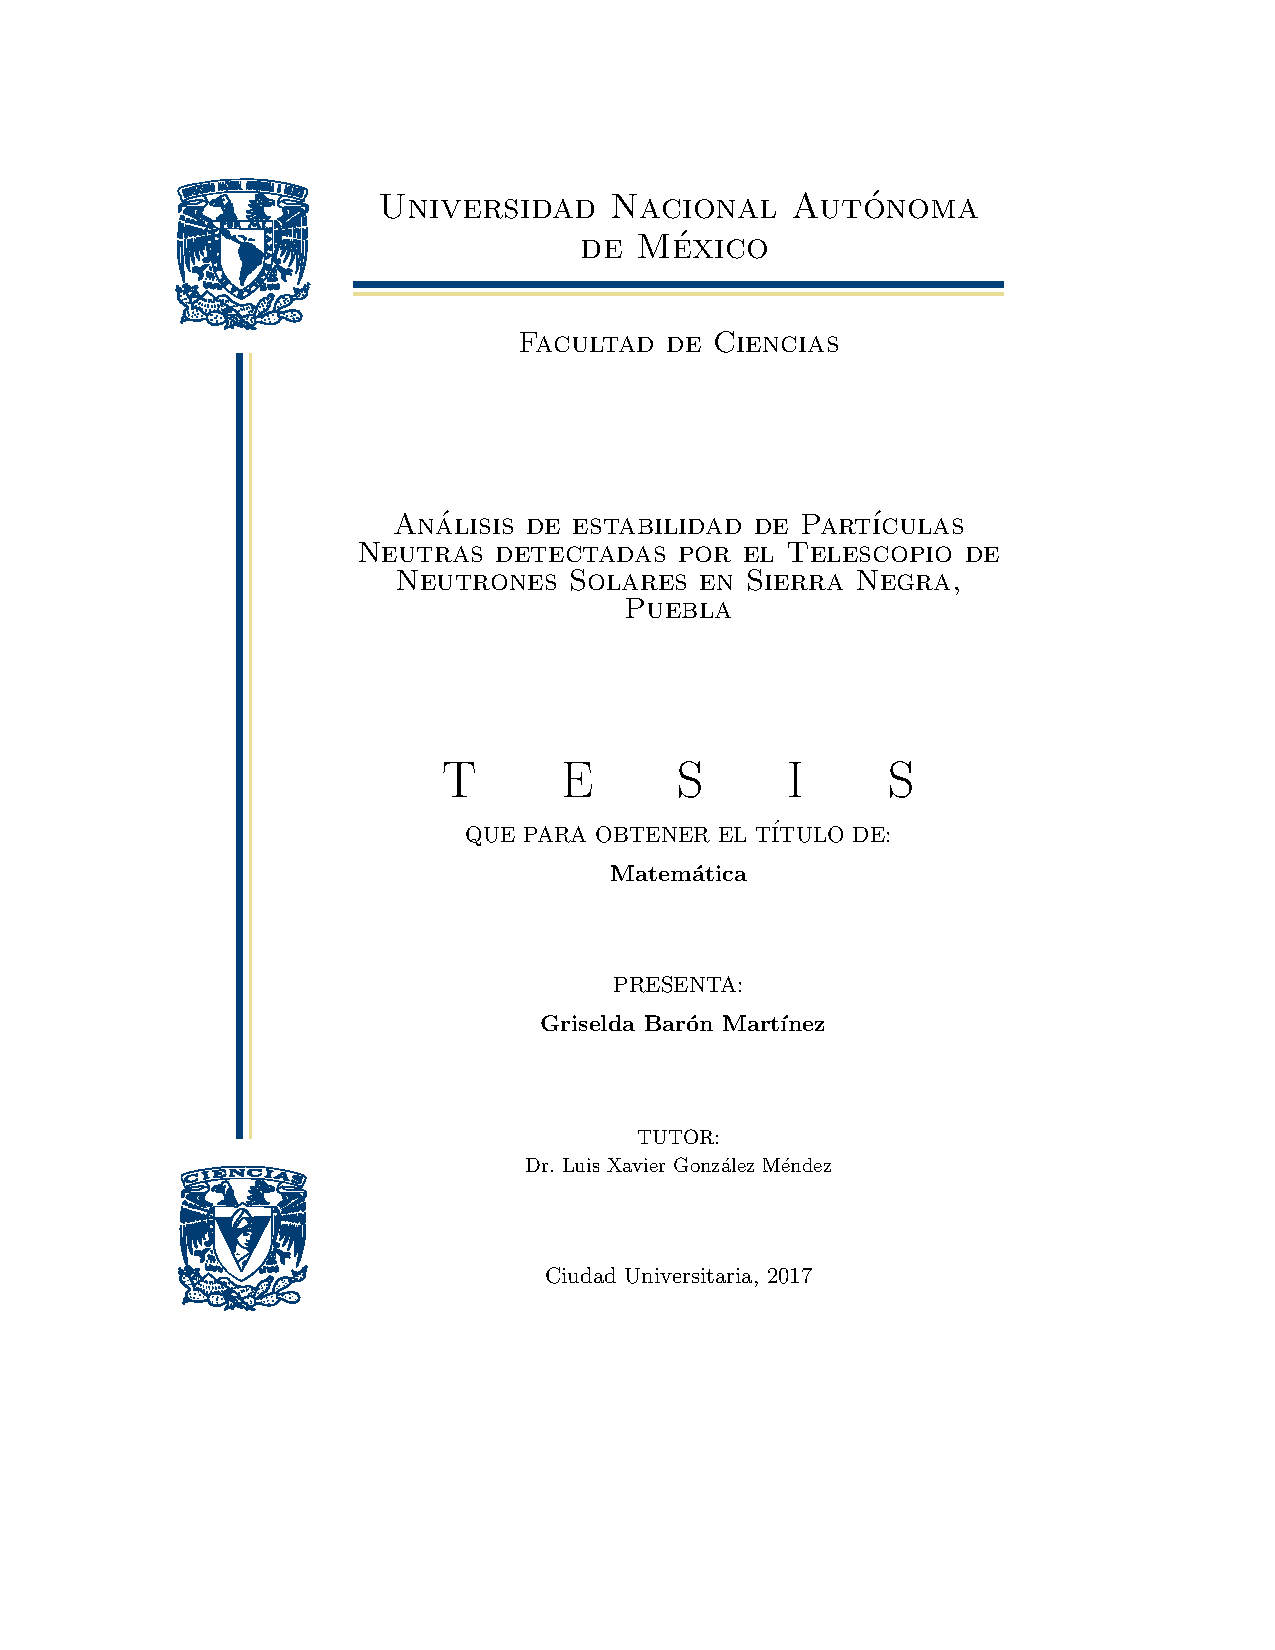
\includepdf{portada.pdf}									% Se redefinió este comando en el archivo de la clase para generar automáticamente la portada a partir de los datos

%%%%%%%%%%%%%%%%%%%%%%%%%%%%%%%%%%%%%%%%%%%%%%%%%%%%%
%                  PRÓLOGO                          %
%%%%%%%%%%%%%%%%%%%%%%%%%%%%%%%%%%%%%%%%%%%%%%%%%%%%%
\frontmatter
%\section*{}
\thispagestyle{empty}
\setlength\epigraphrule{1pt}
\begin{dedication}

\epigraph{\itshape La Estadística tiene que ver con la investigación científica y con cómo hacerla mejor, pero muchos estadísticos piensan que la Estadística es una rama de las matemáticas. Si bien estoy de acuerdo en que los físicos, los químicos, los ingenieros y los estadísticos siempre necesitarán saber matemáticas, su objetivo debe ser hacer mejor física, mejor química, mejor ingeniería y, en el caso de la Estadística, mejor investigación científica. Que esto implique usar muchas o pocas matemáticas en un estudio determinado, es una cuestión puramente incidental.}{\textit{George E. P. Box}}

\end{dedication}








%\begin{dedication}

Con todo cariño y amor a mis padres y hermanos.\\
A la Facultad de Ciencias y a la Universidad Nacional Autónoma de México,\\
por la formación que me han dado. Es gracias a ustedes que es posible el presente trabajo.\\

\end{dedication}
       % Comentar línea si no se usa
%%\chapter*{}
%\pagenumbering{Roman}

\begin{acknowledgements}
\setlength\epigraphrule{0pt}
\thispagestyle{empty}

%\epigraph{\itshape Tlaskamati miak pampa tech nextili ojti uan pampa tij chiua no nemilis ma eli nel kuajkualtsin. \begin{small}Muchas gracias por haberme guiado en este camino y hacer de mi vida la aventura más emocionante.\end{small} }{-Griselda Barón Martínez}

%\vspace{1cm}

Antes que nada quiero agradecer a mis padres y hermanos por el apoyo que me han brindado, especialmente a mi hermana Ana que siempre ha estado conmigo de manera incondicional.\\

Al Dr. Luis Xavier González Méndez por haberme brindado la oportunidad de participar en el proyecto, por la asesoría, el apoyo, la confianza, sus conocimientos, las risas...sin él este trabajo no sería posible.\\

Quiero expresar también mi más sincero agradecimiento al  Dr. José Francisco Valdés Galicia por los datos, el apoyo, las ideas...\\

A PAPIIT por apoyarme durante el servicio social y al Programa Universitario México, Nación Multicultural por facilitarme una beca durante mis estudios y en la realización de esta tesis.\\

A todos los que contribuyen al proyecto R y por su filosofía de software libre. R Development Core Team. R: A language and environment for statistical computing.\\

Gracias Universidad Nacional Autónoma de México y querida Facultad de Ciencias por la excelente educación y hacer de esta travesía la más agradable al mostrarme el maravilloso mundo de las matemáticas. Gracias a todas la personas que, ya sea de manera directa o indirecta, han sido partícipes de este proceso. 

\end{acknowledgements}

\newpage
\thispagestyle{empty}




   % Comentar línea si no se usa 
%\section*{}
\thispagestyle{empty}
\setlength\epigraphrule{1pt}
\begin{dedication}

\epigraph{\itshape La Estadística tiene que ver con la investigación científica y con cómo hacerla mejor, pero muchos estadísticos piensan que la Estadística es una rama de las matemáticas. Si bien estoy de acuerdo en que los físicos, los químicos, los ingenieros y los estadísticos siempre necesitarán saber matemáticas, su objetivo debe ser hacer mejor física, mejor química, mejor ingeniería y, en el caso de la Estadística, mejor investigación científica. Que esto implique usar muchas o pocas matemáticas en un estudio determinado, es una cuestión puramente incidental.}{\textit{George E. P. Box}}

\end{dedication}








%% ******************************* Thesis Declaration ********************************

%\begin{declaration}
%
%Por la presente declaro que, salvo cuando se haga referencia específica al trabajo de otras personas, el contenido de esta tesis es original y no se ha presentado total o parcialmente para su consideración para cualquier otro título o grado en esta o cualquier otra Universidad. Esta tesis es resultado de mi propio trabajo y no incluye nada que sea el resultado de algún trabajo realizado en colaboración, salvo que se indique específicamente en el texto. 
%% Author and date will be inserted automatically from thesis.tex
%
%
%\end{declaration}
           % Comentar línea si no se usa

%%%%%%%%%%%%%%%%%%%%%%%%%%%%%%%%%%%%%%%%%%%%%%%%%%%%%
%                   ÍNDICES                         %
%%%%%%%%%%%%%%%%%%%%%%%%%%%%%%%%%%%%%%%%%%%%%%%%%%%%%
%Esta sección genera el índice
\setcounter{secnumdepth}{3} % organisational level that receives a numbers
\setcounter{tocdepth}{3}    % print table of contents for level 3
\tableofcontents          % Genera el índice 
%: ----------------------- list of figures/tables ------------------------

\listoffigures           % Genera el ínidce de figuras, comentar línea si no se usa

\listoftables               % Genera índice de tablas, comentar línea si no se usa

% Thesis Abstract -----------------------------------------------------


%\begin{abstractslong}    %uncommenting this line, gives a different abstract heading

\begin{abstracts}        %this creates the heading for the abstract page
\addcontentsline{toc}{chapter}{\textbf{Resumen}}
%\markboth{RESUMEN}{RESUMEN}

El Telescopio de Neutrones Solares (TNS) de México se encuentra instalado en la cima del volcán Sierra Negra, Puebla, a 4580 m s.n.m. y está operando desde el año 2004. El TNS cuenta con ocho canales de deposición de energía (E) de partículas incidentes que corresponden a $E\geq 30 \,\, MeV$, $60 \,\, MeV$, $90 \,\, MeV$ y $120 \,\, MeV$, cuatro de éstos canales corresponden a partículas cargadas y los otros cuatro a partículas neutras. Además de medir el fondo de rayos cósmicos galácticos, el TNS tiene la capacidad de detectar la energía y dirección de arribo del flujo de neutrones solares.\\

La base de datos del TNS cuenta hasta la fecha con 13 años de información sobre la detección de rayos cósmicos. En este trabajo se presenta un análisis detallado de estabilidad estadística para la serie total de datos registrados en los canales de partículas neutras desde el año 2004 hasta el año 2016, con una razón de conteo de 10 segundos. Para este análisis se utilizó el software estadístico R, donde se muestran los principales códigos ejecutados.\\

Una vez que se tienen los datos limpios y ordenados se procede con el análisis estadístico y gráfico para después pasar a la interpretación del análisis. Así, este trabajo muestra las variaciones que se han presentado en los registros de partículas neutras para conocer la calidad de los datos detectados y las distintas influencias electrónicas, eléctricas y de fenómenos de actividad atmosférica que han generado cambios en la estadística anual del TNS. Se da a conocer la señal total del detector y cómo ha variado a lo largo del tiempo. De esta manera, el análisis nos permite asegurar que se está trabajando con datos confiables para realizar los estudios básicos de física solar y poder conocer y diferenciar las afectaciones de los fenómenos puramente eléctrico-electrónicos y/o de otra índole.


\end{abstracts}
%\end{abstractlongs}


% ----------------------------------------------------------------------                   % Comentar línea si no se usa

% this file is called up by thesis.tex
% content in this file will be fed into the main document
%----------------------- introduction file header -----------------------
%%%%%%%%%%%%%%%%%%%%%%%%%%%%%%%%%%%%%%%%%%%%%%%%%%%%%%%%%%%%%%%%%%%%%%%%%
%  Capítulo 1: Introducción- DEFINIR OBJETIVOS DE LA TESIS              %
%%%%%%%%%%%%%%%%%%%%%%%%%%%%%%%%%%%%%%%%%%%%%%%%%%%%%%%%%%%%%%%%%%%%%%%%%

\chapter{Introducción}\label{cap.intro}
\markboth{INTRODUCCIÓN}{INTRODUCCIÓN}


%: ----------------------- HELP: latex document organisation
% the commands below help you to subdivide and organise your thesis
%    \chapter{}       = level 1, top level
%    \section{}       = level 2
%    \subsection{}    = level 3
%    \subsubsection{} = level 4
%%%%%%%%%%%%%%%%%%%%%%%%%%%%%%%%%%%%%%%%%%%%%%%%%%%%%%%%%%%%%%%%%%%%%%%%%
%                           Presentación                                %
%%%%%%%%%%%%%%%%%%%%%%%%%%%%%%%%%%%%%%%%%%%%%%%%%%%%%%%%%%%%%%%%%%%%%%%%%

La superficie de nuestro planeta es bombardeada contínuamente por pequeñas y misteriosas partículas que viajan a través del espacio. Estas partículas son los rayos cósmicos que provienen del Sol y de fuera del Sistema Solar. Desde su descubrimiento en 1912 por el físico austriaco Victor Franz Hess\footnote{Galardonado con el Premio Nobel de Física en 1936.} y hasta el descubrimiento del antiprotón por un acelerador de partículas en 1955, la radiación cósmica ha sido el instrumento científico más importante para avanzar en el estudio de las propiedades de las partículas subatómicas\cite{rev}.\\

Los rayos cósmicos son principalmente núcleos atómicos, despojados de sus electrones por los procesos de aceleración en la interacción desde la fuente hasta la Tierra. Hay tres tipos de rayos cósmicos: los galácticos, anómalos y solares. Los \emph{rayos cósmicos galácticos} son de  energía muy alta (hasta $10^{20}\, eV$) y la mayor parte de ésta se genera a partir del nacimiento de las supernovas. Los \emph{rayos cósmicos anómalos} se originan en el medio interplanetario y se denominan así porque su composición es inusual; no sigue las abundancias naturales predichas para los diferentes isótopos\footnote{Núcleos del mismo elemento que tienen diferente número de neutrones.}\cite{cosmicray}. Hoy en día se sabe que en la atmósfera solar también se producen una gran cantidad de partículas a las que llamamos \emph{rayos cósmicos solares} y cuya energía puede ser del orden de $10^{10}$\,$eV$\footnote{Los $eV$ (electrón-volts) son unidades que miden la energía cinética adquirida por un electrón cuando es acelerado en un campo eléctrico producido por una diferencia de potencial de un volt. Ver más en \cite{mensajeros} y \cite{brunorossi}.}\cite{TNS}. El Sol, además de ser nuestra principal fuente de luz y calor, es el mayor acelerador de partículas del Sistema Solar, el cual es capaz de producir neutrones relativistas, principalmente en fulguraciones clase~X (véase el apéndice A).\\


Una fulguración solar es una explosión en el Sol que ocurre cuando la energía almacenada en campos magnéticos intensos se libera repentinamente. Esta explosión genera muchas veces una gran cantidad de partículas de energía muy alta, la mayor parte son partículas cargadas (electrones, protones y núcleos de elementos más pesados), éstas son desviadas por campos magnéticos en el sitio de aceleración, en el medio interplanetario y en el campo geomagnético. De esta forma, al llegar a la Tierra, la información física relevante se pierde. Las partículas neutras, al no ser afectadas por el campo magnético interplanetario, conservan información relevante para comprender  y calcular el espectro de los iones y su tiempo de producción.\cite{TNS}.\\
 
Los neutrones solares contienen información importante sobre los mecanismos de aceleración de iones en la atmósfera del Sol\cite{watanab}. Con base en que el tiempo de vida media de los neutrones libres es de 886 segundos, tienen que ser relativistas\footnote{$E > m_{o} c^2$ donde $m_{o}$ es la masa en reposo de la partícula y c es la velocidad de la luz en el vacío.} para que sean detectados en tierra.\\
 
El mecanismo de aceleración de los electrones ha sido estudiado mediante las observaciones con rayos X y rayos gamma (rayos $\gamma$), mientras que el de los iones aún no se comprende totalmente\cite{TNS}. La información de la aceleración de iones se transfiere a los neutrones solares y las lineas de rayos $\gamma$ que son generados por las reacciones nucleares de las partículas aceleradas con núcleos en la atmósfera solar\cite{hua1987solar}. De aquí la importancia de detectar neutrones solares.\\
 
Es necesario conocer la energía de los neutrones solares para calcular el tiempo de aceleración y saber si la aceleración de partículas es gradual o impulsiva, para ello se debe tener registro simultáneo de neutrones solares en tierra y de las emisiones rayos X y rayos $\gamma$ en el espacio\cite{TNS}.\\ 
 
 En el instituto de Geofísica de la UNAM se detectan rayos cósmicos con energías desde los 8.2 GeV\footnote{Rigidez umbral. Véase el \emph{capítulo 1}} con un instrumento que se conoce como Monitor de Neutrones\footnote{El MN instalado en C.U. es considerado uno de los detectores de neutrones más estables del mundo\cite{geo}.} (MN)\cite{geo}. El MN mide el flujo de rayos cósmicos galácticos y las variaciones debidas a las emisiones de la actividad del Sol, además de rayos cósmicos solares que se emiten cuando hay fulguraciones extremas. El MN tiene una alta sensibilidad, pero no puede conocer la dirección de arribo y energía de las partículas incidentes y no discrimina entre protones y neutrones. Por esta razón, es necesario usar un equipo nuevo especializado en la detección de neutrones solares.\\

El Telescopio de Neutrones Solares (TNS) es capaz de medir el flujo de neutrones solares, la energía primaria y diferenciar entre neutrones y protones. El nombre de telescopio se debe a que además de la capacidad mencionada anteriormente, mide la dirección de arribo de las partículas incidentes. Existe una red mundial de TNS instalados en altas montañas (Armenia, Bolivia, China, Hawai, Japón, Suiza y México). En México se instaló en la cima del volcán Sierra Negra, Puebla, en colaboración con el STELab (Solar Terrestrial Environment Laboratory) de la Universidad de Nagoya, Japón\cite{valdes}. Ha estado funcionando de manera casi continua desde julio de 2004 y ha registrado dos eventos de neutrones solares producidos en la fulguración del 7 de septiembre de 2005 y el 8 de julio de 2014\cite{Luisx,murakii}.\\

Desde 2004 hasta 2016 se tienen 13 años de registro de la detección del TNS con cuatro canales de deposición de energía. Debido al interés por observar y comprender los fenómenos y mecanismos físicos que produce el Sol, es de gran importancia hacer un análisis estadístico detallado y estudiar la estabilidad de los datos a lo largo del tiempo antes de hacer estudios de física solar. El análisis se realiza para datos de los cuatro canales de energía que registran partículas neutras, con el uso del software estadístico R.\\


Este trabajo está estructurado en 4 capítulos. En el capítulo 1 se da una breve introducción a los rayos cósmicos, en particular a los rayos cósmicos solares y se explican las principales variaciones observadas.

En el capítulo 2 se muestra la red mundial de Telescopios de Neutrones Solares; en particular las características del TNS instalado en Sierra Negra, así como el diseño, canales y capacidad de detección. También se dan las características de los datos registrados por el TNS en Sierra Negra, ya que durante los 13 de años de detección se cambió la programación del registro de datos debido a ajustes y calibración del equipo.\\ 

Con el avance de la tecnología, el proceso de adquisición de datos se ha vuelto más eficiente, esto implica gran cantidad de almacenamiento de datos. Para manipular, analizar y extraer información importante de estos datos es necesario hacer uso de algún software para programación estadística. Por esta razón, el capítulo 3 se dedica al lenguaje R, el cual se usó para llevar a cabo el análisis estadístico del presente trabajo. Se muestran los códigos programados; desde la importación y limpieza de los datos del TNS, hasta el análisis gráfico y estadístico.\\

El capitulo 4 muestra un análisis detallado de las distintas variaciones que ha presentado el flujo de partículas neutras durante 13 años para los cuatro canales de energía con anticoincidencia electrónica.\\

Finalmente se exponen las conclusiones del análisis estadístico y se muestra la señal total del detector (2004-2016).             % ~10 páginas - Explicar el propósito de la tesis
%%%%%%%%%%%%%%%%%%%%%%%%%%%%%%%%%%%%%%%%%%%%%%%%%%%%%
%                   CONTENIDO                       %
%%%%%%%%%%%%%%%%%%%%%%%%%%%%%%%%%%%%%%%%%%%%%%%%%%%%%
% the main text starts here with the introduction, 1st chapter,...
\mainmatter
\def\baselinestretch{1.5}                   % Interlineado de 1.5
\chapter{Los rayos cósmicos}

\section{¿Qué son los rayos cósmicos?}

Los rayos cósmicos son núcleos ionizados mediante procesos de aceleración que viajan a través de la Vía Láctea, incluyendo el sistema solar. Se producen en estrellas, remanentes de supernovas, núcleos activos de galaxias y otros objetos astrofísicos. La composición de los rayos cósmicos es de aprox 93\% de protones, 6.3\% de partículas alfa y 0.7\% son núcleos de elementos más pesados. La pregunta fundamental es, ¿dónde se originan? y en particular, ¿como es que son aceleradas a tan altas energías?. La respuesta  a la pregunta del origen de los rayos cosmicos todavía no es totalmente conocido. Es claro, sin embargo, que casi todos ellos vienen desde fuera del sistema solar, pero desde dentro de la galaxia\cite{thomas}.\\

Se denominan rayos cósmicos primarios a las partículas que inciden en la atmósfera terrestre procedentes del espacio, compuestos principalmente de protones y partículas alfa. Al interactuar con un núcleo atmosférico producen una cascada de partículas compuesta por rayos $\gamma$, electrones, muones,etc, que son llamados rayos cósmicos secundarios\cite{spatium}.\\

El \emph{espectro de energía} de la radiación cósmica primaria describe cómo están distribuidas con respecto a la energía. En la Figura \ref{espectro}

\begin{figure}[H]
  \centering
    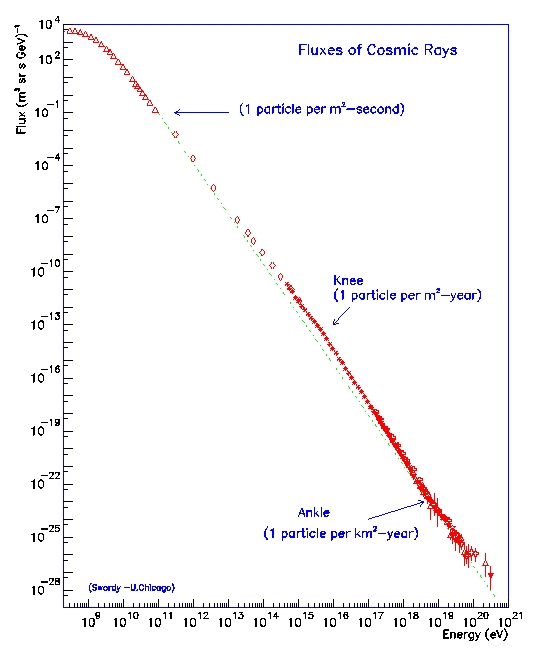
\includegraphics[scale=0.60]{Capitulo1/figs/esp.jpg}      %Ruta completa de la imagen, porque se compila desde el archivo tesis.tex
  \caption{Espectro de energía de rayos cósmicos.}            %Pie de imagen
  \label{espectro}                            %nombre de referencia
\end{figure}

Existe un gran número de mediciones y estudios del sector del
espectro con energías menores al tobillo; la existencia de la rodilla
está aún incompletamente explicada. Para energías mayores al tobillo
los rayos cósmicos ya no pueden ser confinados por el campo
magnético de la Vía Láctea y provienen de todas las direcciones por
igual. Esto indica que estos rayos cósmicos proceden de fuera de la
Galaxia. Además, las mediciones del grupo experimental Fly's Eye
sugieren que los rayos bajo el tobillo son principalmente núcleos de
átomos pesados(mayormente Fe), mientras que los eventos sobre el
tobillo son exclusivamente protones y neutrones. Esto es consistente
con la hipótesis de que los rayos supra-tobillos son extragalácticos, ya
que los núcleos pesados con energías superiores a 4x1018 eV no
podrían sobrevivir un viaje extragaláctico debido al roce con el Fondo
de Radiación Cósmica (FRC), mecanismo que se describirá más
adelante.



La Heliosfera es responsable de afectar a las partículas con energías que van desde los 109 eV a los 1015 eV, en la región del espectro conocida como ``rodilla", por debajo de esta zona, los RC galácticos son la contribución dominante. Las partículas con energías de \~1015-1017 eV son probablemente aceleradas por mecanismos de choques rápidos como los remanentes de supernovas.
Las partículas con energías superiores son llamadas “de ultra alta energía”, poseen radios de giro comparables con el radio de nuestra galaxia, son muy poco abundantes en comparación a los RC galácticos y su fuente aún no está plenamente confirmada, debido a esto, a menudo se les considera RC extra-galácticos. Alrededor de 1020 eV, el espectro comienza a aplanarse de nuevo, formando la región conocida como ``tobillo".

Durante muchos años se ha observado que la intensidad de los rayos cósmicos medida en la Tierra experimenta variaciones periódicas en función a las emisiones de la actividad del Sol, es decir, estas variaciones son producidas por la \emph{modulación solar}\cite{grieder}. La actividad solar modula el flujo de rayos cósmicos detectados en tierra. Entre las variaciones observadas en la radiación cósmica y que son influenciadas por el Sol se encuentran:

\begin{enumerate}[a)]
 \item \emph{La variación de 11 años}
 \item \emph{El decrecimiento Forbush}
 \item \emph{La variación diurna}
 \end{enumerate}

 
La \emph{variación de 11 años} está sujeta a una variación periódica debida al ciclo solar promedio de 11 años. Existe una anti-correlación entre los rayos cósmicos detectados y el número de manchas solares. Como el número de manchas solares es un indicador de la actividad solar, a mayor número de manchas, mayor actividad y emisiones en el Sol. Las emisiones de la actividad del Sol permean todo el Sistema Solar con líneas de campo magnético, las cuales desvían a los rayos cósmicos que ingresan. Cuando el Sol se encuentra con baja actividad, las emisiones son menos intensas y permiten que el flujo de rayos cósmicos galácticos se incremente. Por lo tanto, a mínimo número de manchas, menor cantidad de emisiones solares y mayor el flujo de rayos cósmicos detectados, con un retardo de aproximadamente 1 o 2 años\cite{stanev}. En la figura \ref{sunspot} se puede ver la anti-correlación entre el número de manchas solares observados por Solar Influences Data Analysis Center (SIDC)  y las cuentas del monitor de neutrones de Oulu.\\ 

El \emph{decrecimiento Forbush}, llamado así en honor al físico estadounidense Scott E. Forbush, es el decrecimiento repentino de la intensidad de la radiación cósmica hasta en un 10\% y ocasionalmente 20 o 30\% en el lapso de unas cuantas horas. Una vez que la intensidad ha llegado a un mínimo empieza a recuperarse gradualmente, lo cual puede durar varias horas, días o incluso semanas.\\

\begin{figure}[H]
\centering
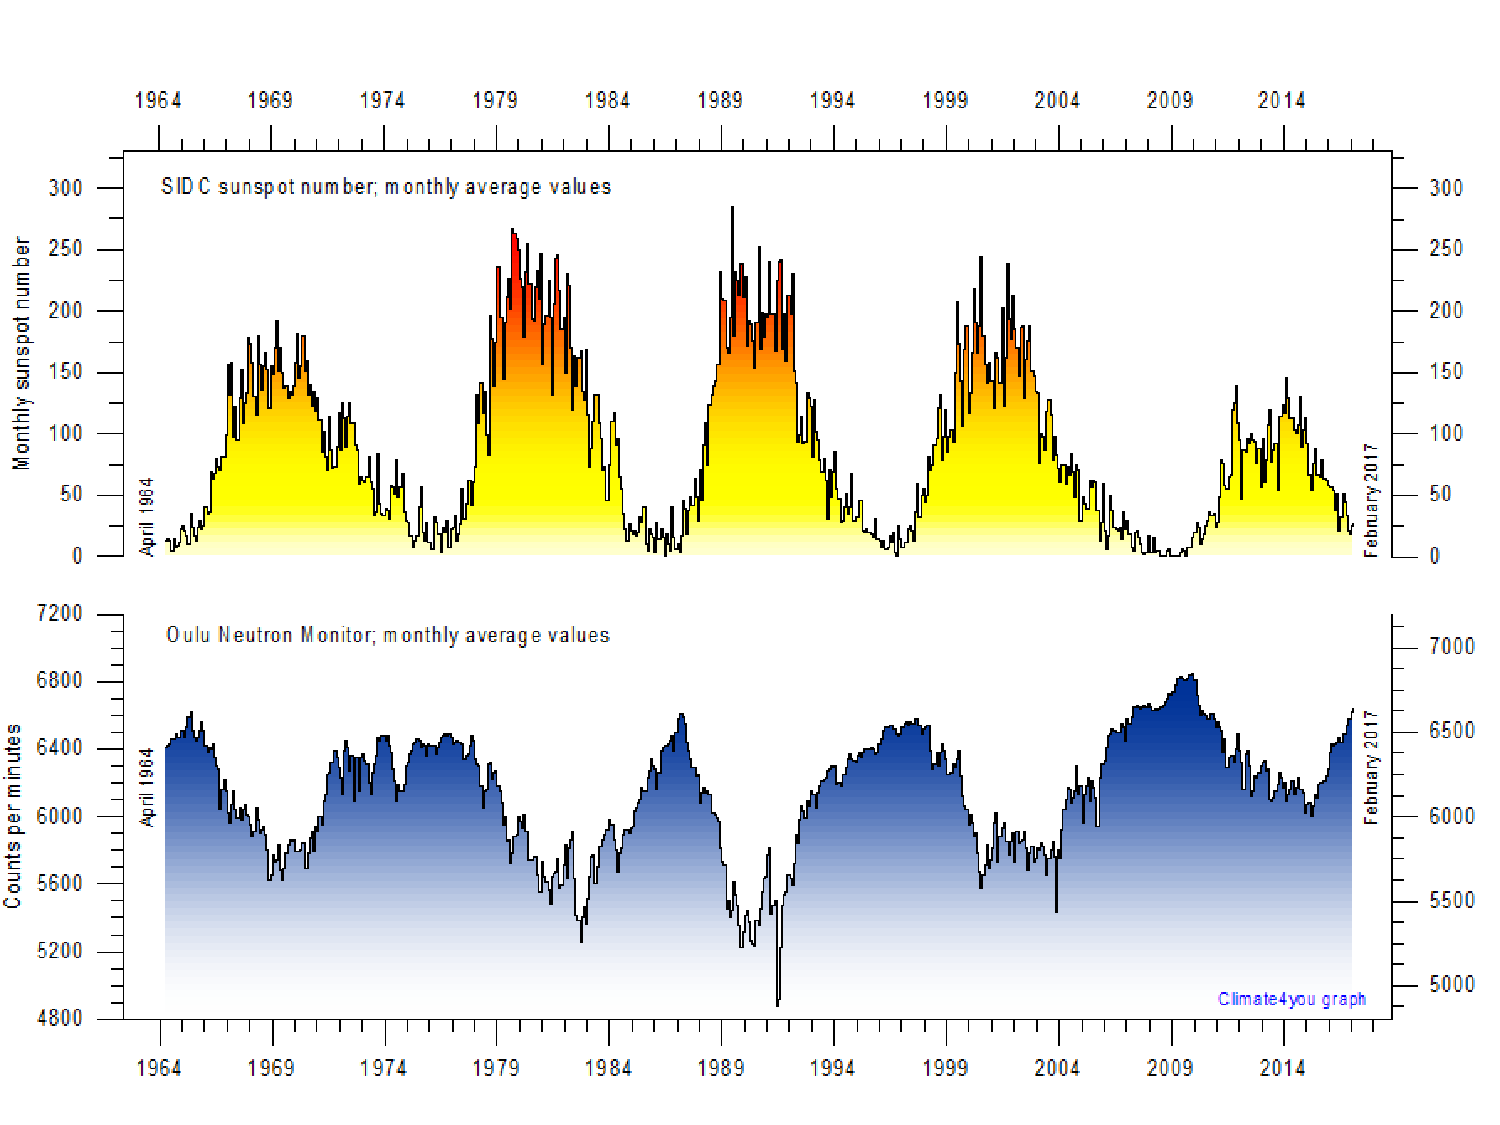
\includegraphics[scale=0.50]{Capitulo1/figs/cr_vs_sunspots.pdf}
\caption{Observaciones mensuales del número manchas solares (Solar Influences Data Analysis Center (SIDC)) desde abril de 1964, y medias mensuales de las cuentas del monitor de neutrones de Oulu (Finlandia), ajustados por presión barométrica y eficiencia. Actualización: 1 de marzo de 2017.}
\label{sunspot} 
\end{figure}
 
Aún se estudian los mecanismos y procesos de generación de los decrecimientos Forbush y se sabe que son un efecto de las líneas de campo magnético asociadas con las emisiones solares. En el momento que ocurre una ráfaga solar o una eyección de masa coronal de una región activa del Sol, la nube de plasma eyectada puede tener una velocidad más alta que el viento solar normal, lo cual produce una discontinuidad brusca conocida como \emph{onda de choque}. La onda de choque forma un ``contenedor" magnético con una intensidad de campo relativamente alta. Si la Tierra se encuentra dentro de este contenedor, la radiación cósmica es desviada en función a su energía y no ingresa a la atmósfera; a medida que esta onda se aleja, menos será la influencia sobre las partículas\cite{grieder,mensajeros}. En la figura \ref{forbush} se muestra un decrecimiento forbush detectado por el monitor de neutrones del Observatorio de Rayos Cósmicos de la Ciudad de México.\\

\begin{figure}[H]
\centering
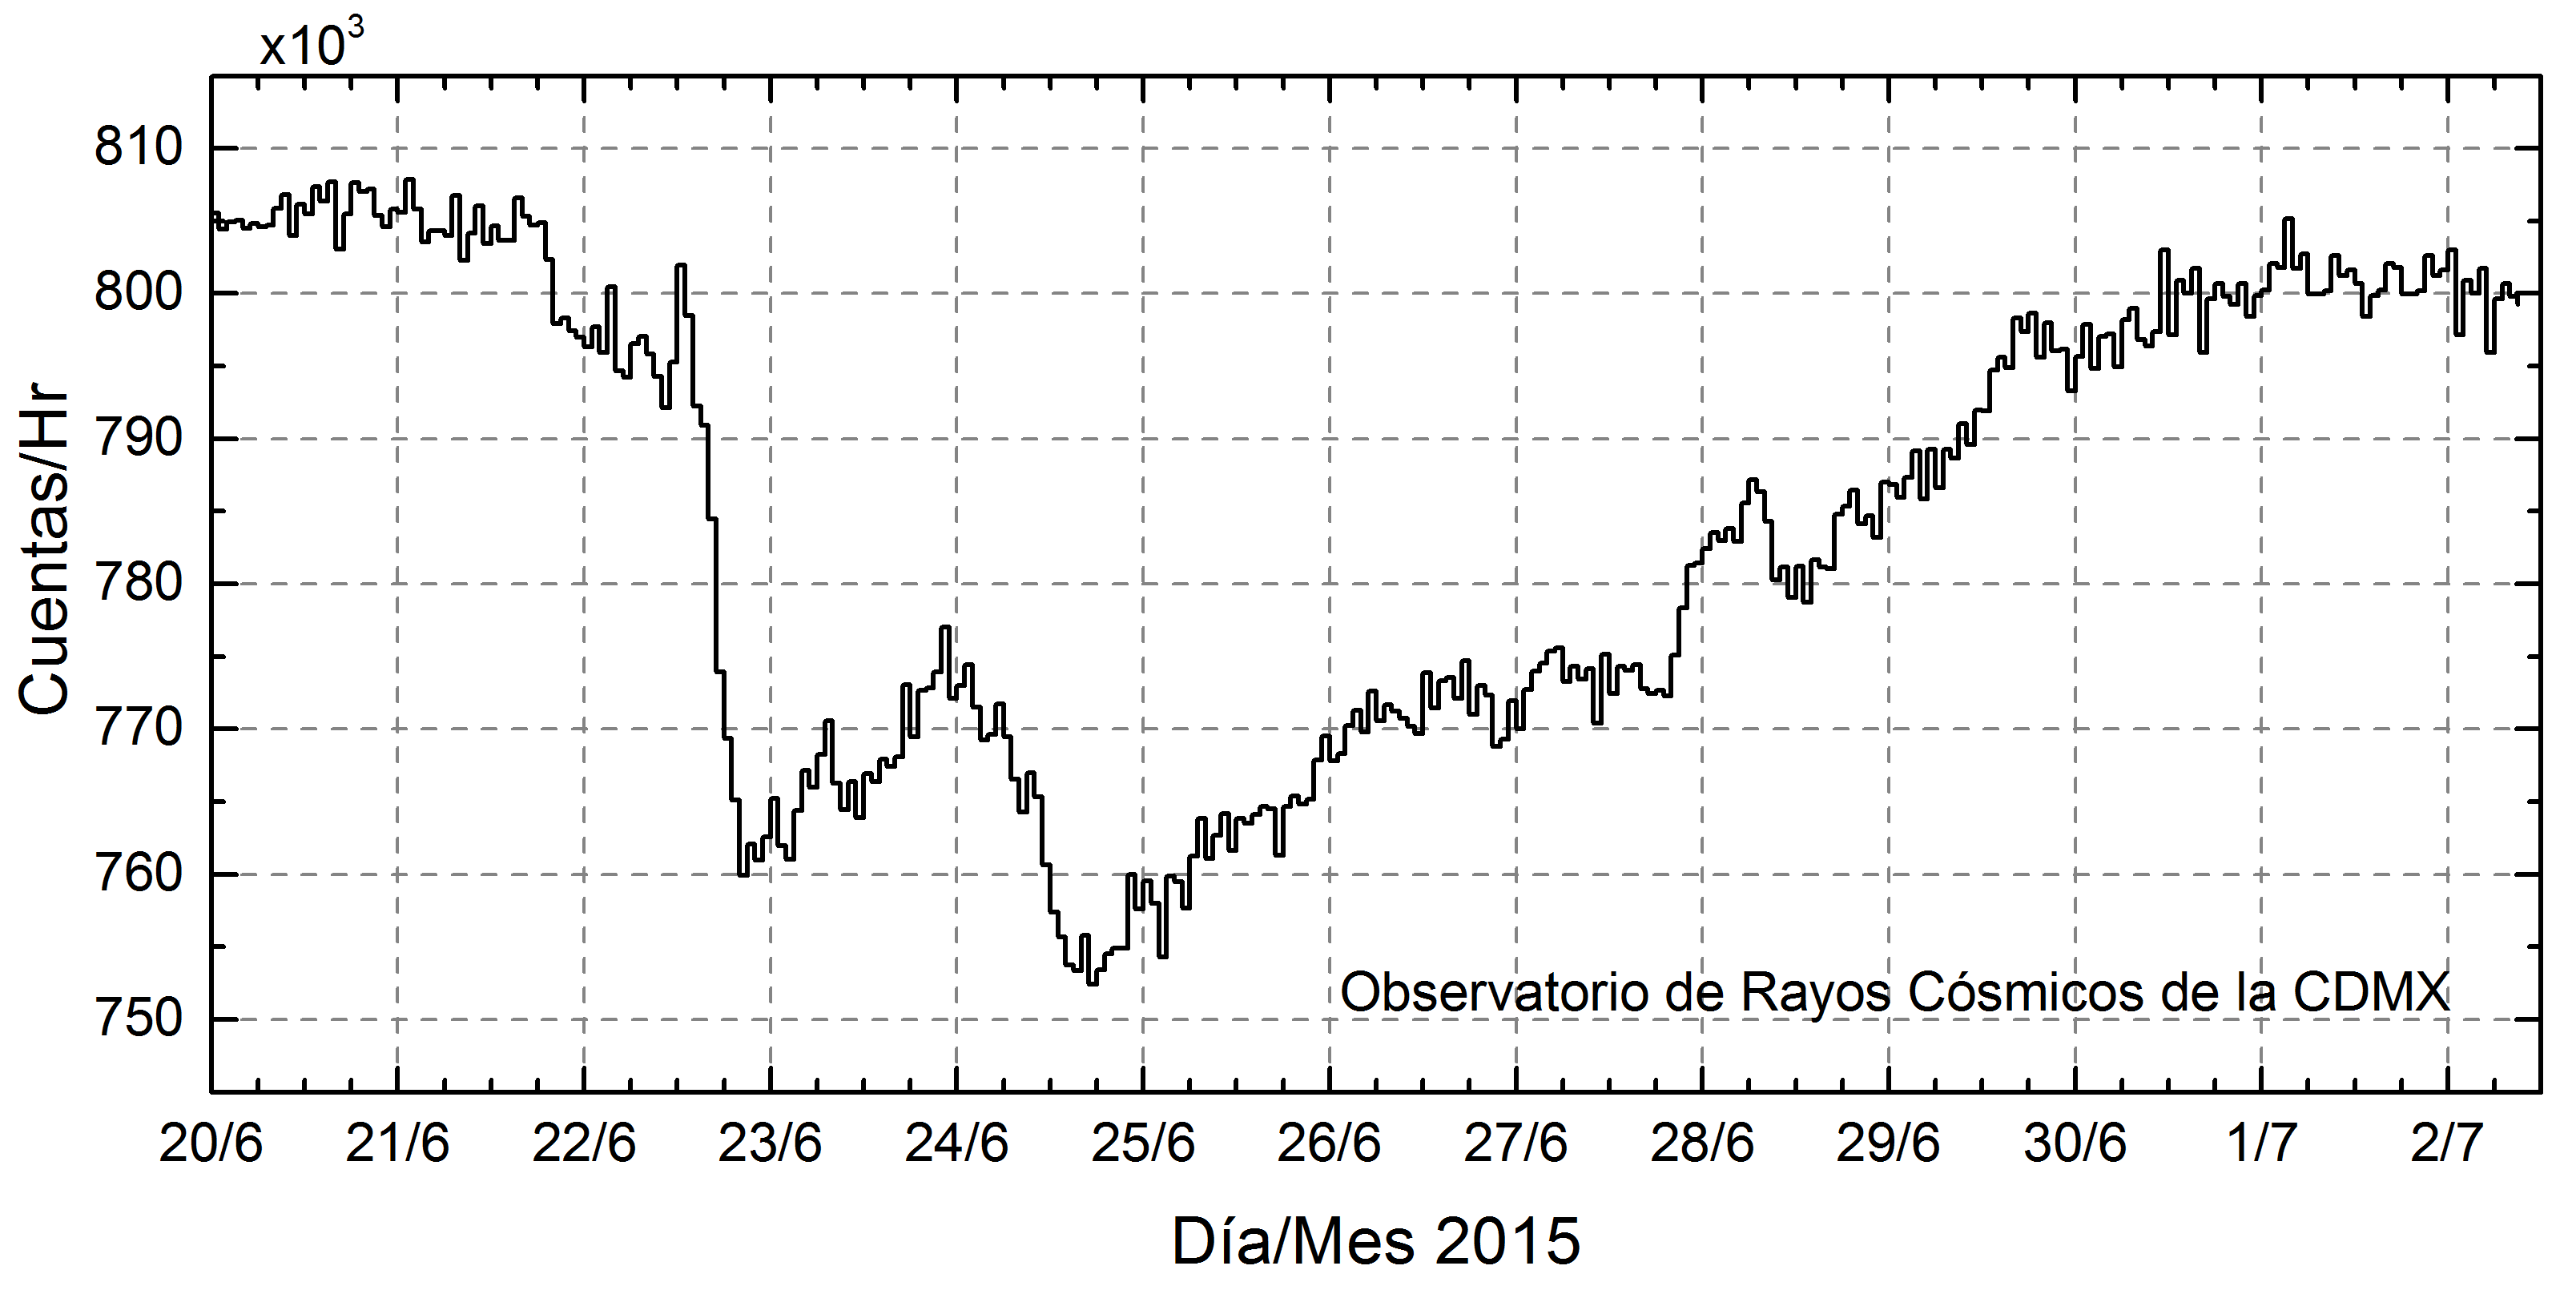
\includegraphics[scale=0.50]{Capitulo1/figs/Decrecimiento_Forbush.png}
\caption{Decrecimiento Forbush detectado por  el monitor de neutrones de la Ciudad de México el 22 de  junio de 2015.}
\label{forbush} 
\end{figure}

La \emph{variación diurna} es una variación periódica en la intensidad de la radiación cósmica. Tiene una  periodicidad de un día solar, que es el tiempo que tarda la Tierra en dar una vuelta sobre su propio eje. El campo magnético gira con el Sol y como los rayos cósmicos giran en espiral alrededor de las líneas de campo, las partículas que se mueven en la misma dirección que la Tierra a lo largo de su órbita tienen un exceso de flujo de aproximadamente 0.7\% comparado con la dirección opuesta\cite{grieder}. Esta variación, al ser observada en una estación terrestre, presenta un máximo y un mínimo de intensidad durante  las 24 horas. El máximo ocurre alrededor de la 15 y 18 hrs en tiempo local y un mínimo sobre las 3 de la mañana. Cuando se hacen las correcciones necesarias para tomar en cuenta los efectos del campo geomagnético sobre las partículas de la radiación cósmica, se observa que siempre el máximo de la intensidad se encuentra alrededor de las 18 horas en tiempo local\cite{mensajeros}. 
\chapter{El TNS y la red mundial de observatorios}
Entender el mecanismo de aceleración de partículas es un tema trascendental en la astrofísica, más aún el proceso de aceleración de iones que todavía no se comprende perfectamente. El Sol, siendo el acelerador natural de partículas más cercano, provee de grandes oportunidades para estudiar este proceso\cite{ValdesGalicia2009565}. El mejor camino para entender el mecanismo de aceleración de iones en la atmósfera solar es usando datos obtenidos por los detectores de neutrones y rayos gama\cite{murak}.\\

Los monitores de neutrones tienen cuentas muy elevadas debido a su alta sensibilidad y no pueden diferenciar la dirección de arribo de las partículas incidentes\cite{Tsuchiya2001183}. Tampoco resuelven la energía de las partículas y no discriminan entre neutrones y protones. Por esta razón, es necesario el uso de un nuevo equipo para resolver los inconvenientes mencionados. El Telescopio de Neutrones Solares \textsc{(TNS)} puede diferenciar entre neutrones y protones, y medir el flujo neutrones solares, su energía y dirección de arribo de las partículas incidentes\cite{valdes,TNS}.\\

En este capítulo se muestra la red mundial de Telescopios de Neutrones Solares y se describen las carácteristicas del TNS instalado en Sierra Negra, así como la estructura de los datos registrados. \\

\section{Red mundial de TNS}

Para interpretar cualquier medición de intensidad de radiación cósmica que se realice cerca de la superficie de la tierra se requiere tomar en cuenta la presencia del campo magnético terrestre. El campo geomagnético, así como nos protege de los efectos nocivos, también controla la cantidad de rayos cósmicos que llega a la superficie. Por ejemplo, si apuntamos un detector de rayos cósmicos hacia la dirección vertical, se observará que el detector recibe todas las partículas de rigideces altas, como si no estuviera el campo geomagnético. Sin embargo, si seguimos midiendo el flujo de rigideces magnéticas menores veremos que hay una rigidez debajo de la cual ya no se detecta ninguna partícula, a ésta se le conoce como \emph{rigidez umbral}. Además, si desplazamos el detector vertical desde el ecuador hacia los polos veremos que la rigidez umbral va disminuyendo\cite{mensajeros}. De este modo, los rayos cósmicos que llegan a mayores latitudes magnéticas penetran facilmente a la atmósfera, mientras que los que llegan a bajas latitudes magnéticas requieren más energía para penetrar.\\

Además de la latitud geomagnética y la energía de partículas, la altura a la cual se encuentra el detector también es muy importante; si se ubica a grandes alturas sobre el nivel del mar, el número de cuentas que registre será mayor debido a que la absorción atmosférica de las partículas secundarias disminuye pues hay menos masa\cite{chismes}.\\

Si se quiere tener una mayor eficiencia en la detección de neutrones, los telescopios deben ser colocados muy cerca del ecuador para que el tiempo de exposición a la radiación solar sea más uniforme a lo largo del año y que la rigidez umbral requerida para los iones incidentes sea muy alta. También debe estar localizado a la mayor altura posible para reducir la cantidad de materia que puede interaccionar con los neutrones solares, disminuyendo la posible contaminación de partículas energéticas cargadas. Por lo tanto, los sitios ideales para las mediciones es en lo alto de las montañas.\\

Predecir cuándo habrá un evento de neutrones solares es imposible, por ello se ha instalado una red de telescopios de neutrones solares a diferentes longitudes alrededor del mundo para tener observación del Sol las 24 horas. La red mundial de TNS está construida tomando en cuenta los detalles sobre la localización geográfica para tener una óptima observación. Hasta ahora se han instalado siete detectores de este tipo alrededor del planeta, el más nuevo de ellos es el instalado en México. En la figura \ref{red} se puede ver la localización geográfica de cada TNS, así como el país en el que se encuentra instalado.\\


\begin{figure}[H]
  \centering
    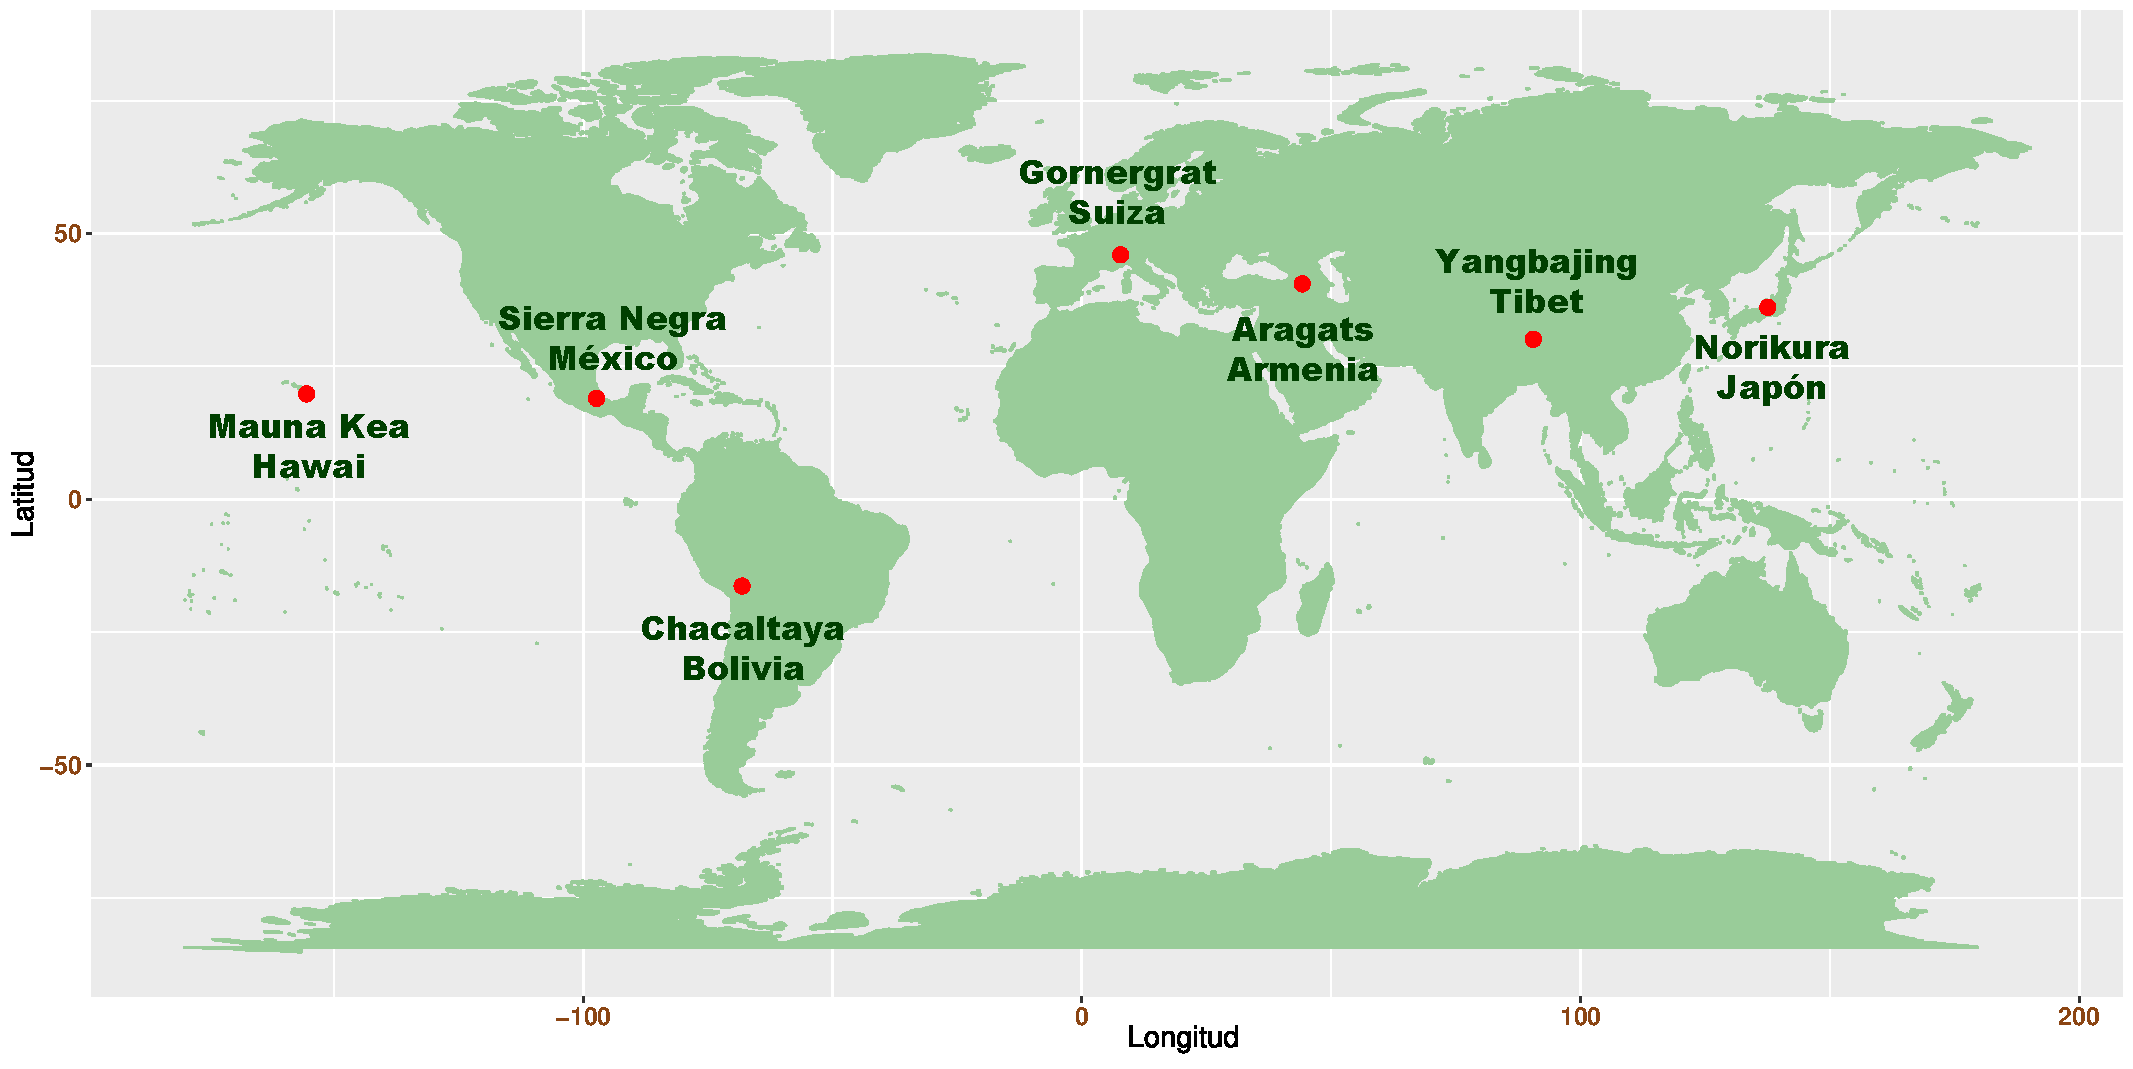
\includegraphics[scale=0.43]{Capitulo2/figs/mapatns.pdf}      %Ruta completa de la imagen, porque se compila desde el archivo tesis.tex
  \caption{Localización geográfica de los TNS alrededor del planeta.}            %Pie de imagen
  \label{red}                            %nombre de referencia
\end{figure}


En la tabla \ref{caractred} se  muestra las coordenadas y altura de los siete TNS  que conforman la red mundial, también la fecha en que se comenzaron a hacer las primeras observaciones. Para ver más características de los TNS se recomienda \textit{Detection efficiency of a new type of solar neutron detector calibrated by an accelerator neutron beam} de H. Tsuchiya \cite{Tsuchiya2001183}.\\

\begin{table}[htb]
\centering
\begin{tabular}{|c|c|c|c|c|}
\hline
{\bf \multirow{2}{*}{Localización}}  & \multirow{2}{*}{{\bf Altura}} & {\bf \multirow{2}{*}{ Longitud}} & {\bf \multirow{2}{*}{Latitud}} & {\bf \multirow{2}{*}{Inicio de la }}\\
  & m.s.n.m &  &  & \bf observación \\
\hline
Gronergrat, Suiza  & 3135 &  $7.8^{\circ}$ E & $46.0^{\circ}$ N & Enero 1998\\
\hline
Aragats, Armenia  & 3200 & $40.5^{\circ}$ E & $44.2^{\circ}$ N & Jun 1997\\
\hline
Yanbajing, Tibet  & 4300 & $90.5^{\circ}$ E & $30.0^{\circ}$ N & Sep 1998\\
\hline
Mt. Norikura, Japón  & 2770 & $137.5^{\circ}$ E & $36.1^{\circ}$ N & Oct 1990\\
\hline
Mauna Kea, Hawaii  & 4200 & $156.3^{\circ}$ W & $19.8^{\circ}$ N & Abr 1997\\
\hline
Sierra Negra, México  & 4580 & $97.3^{\circ}$ W & $19.0^{\circ}$ N & Jul 2004\\
\hline
Chacaltaya, Bolivia & 5250 & $68^{\circ}$ W & $16.2^{\circ}$ S & Sep 1992\\
\hline
\end{tabular}
\caption{Datos de la Red Mundial de TNS.} 
\label{caractred} 
\end{table}

\section{El TNS en Sierra negra}

Sierra Negra es un volcán inactivo localizado en la parte oriental del estado de Puebla, tiene una altura de 4580 m s.n.m., es uno de los picos más altos de la meseta central mexicana. La cima del volcán alberga diversos proyectos astronómicos,\footnote{El Observatorio Solar Mexicano de Gran Altura (OSOMEGA) de la Universidad Nacional Autónoma de México (\url{http://naolinco.geofisica.unam.mx/observatorios/osmega/index.html}). También el Gran Telescopio Milimétrico, un proyecto entre el Instituto Nacional de Astrofísica, Óptica y Electrónica (INAOE) y la Universidad de Massachusetts Amherst (\url{http://www.lmtgtm.org/?lang=es}), entre otros.} uno de ellos es el TNS que forma parte de la red mundial de observatorios.\\

Debido a su localización geográfica, Sierra Negra fue escogido como el mejor lugar para colocar un TNS en México. Además, las condiciones atmosféricas son lo suficientemente moderadas; así que se preserva el flujo de una buena parte de neutrones solares emitidos en fulguraciones. La instalación se llevó a cabo entre el STELab (Solar Terrestrial Environment Laboratory) de la Universidad de Nagoya, Japón y el Instituto de Geofísica de la UNAM.\\

Se puede ver en la figura \ref{red} que el TNS en Sierra Negra está ubicado, longitudinalmente, entre los detectores de Hawai y Chacaltaya, lo cual ayuda a tener en observación al Sol de manera continua, y la combinación de altura/latitud proporciona un tiempo considerable para tal efecto .\\

El TNS fue construido y probado en Marzo de 2003 en Sierra Negra, Puebla ($97.3^{\circ}$ W, $19.0^{\circ}$ N) y ha estado operando desde julio de 2004\cite{geo}. La figura \ref{tns} muestra un esquema del TNS.\\
 
 \begin{figure}[H]
  \centering
    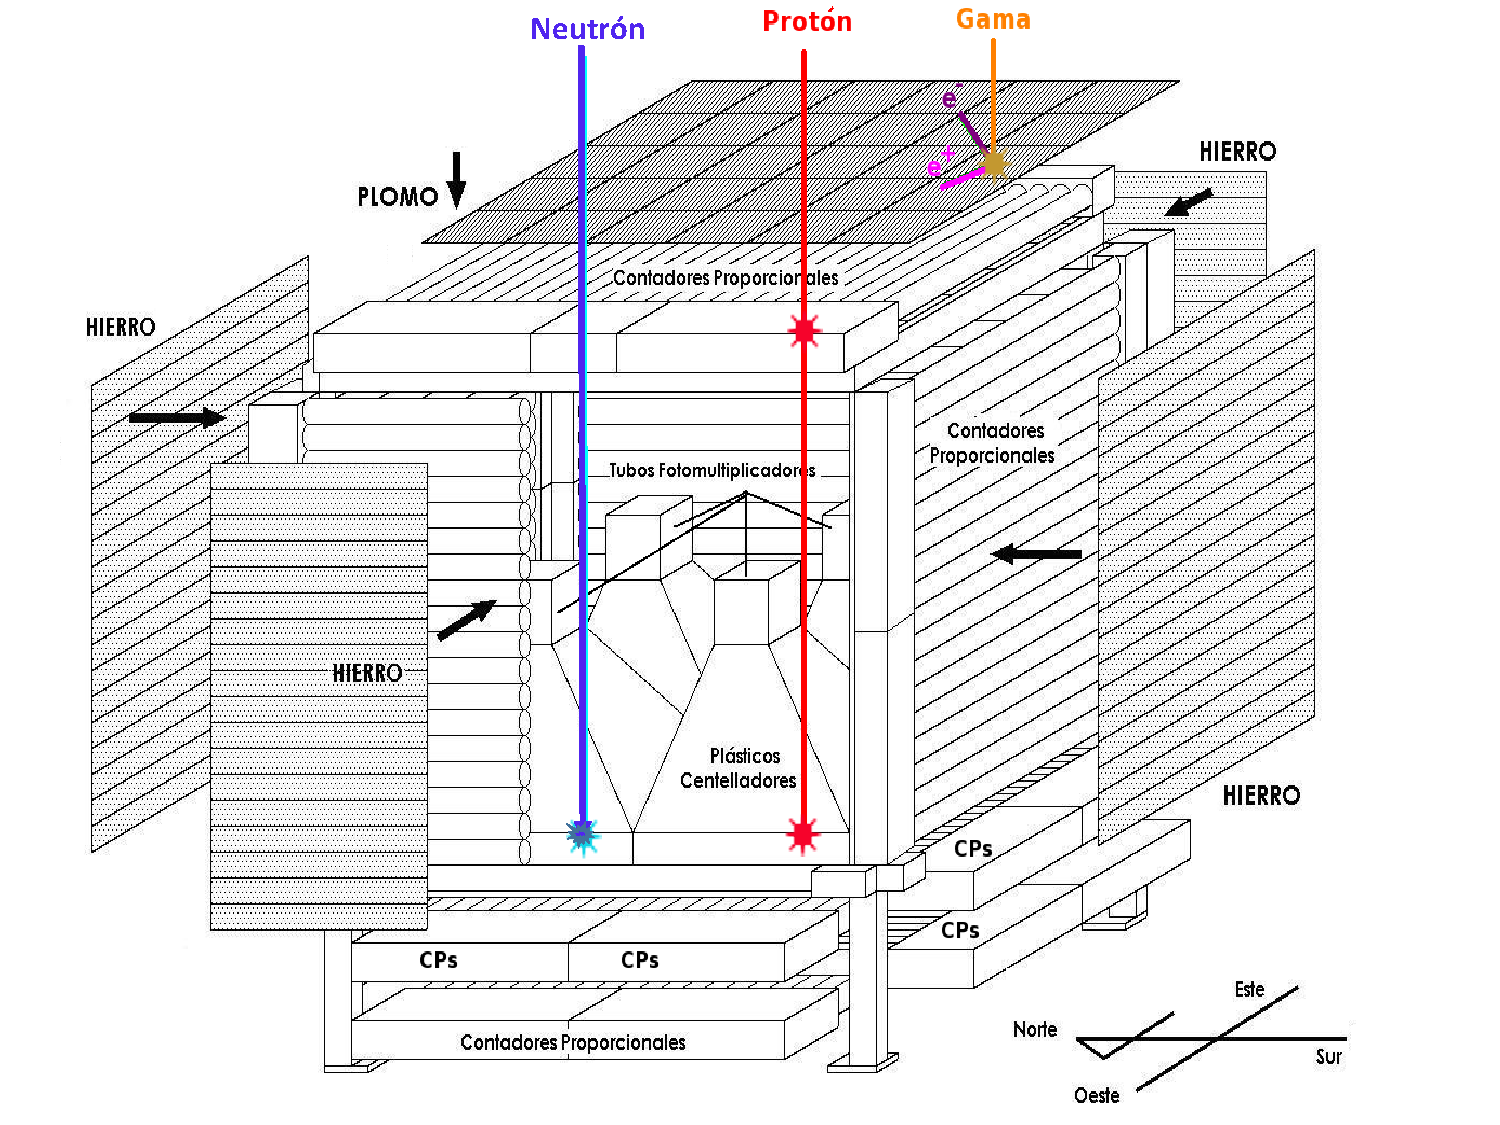
\includegraphics[scale=0.60]{Capitulo2/figs/EsTNS.pdf}      %Ruta completa de la imagen, porque se compila desde el archivo tesis.tex
  \caption{Esquema del TNS instalado en la cima del volcán Sierra Negra, Puebla.}            %Pie de imagen
  \label{tns}                            %nombre de referencia
\end{figure}

El TNS en Sierra Negra consiste de 4 plásticos centelladores (PC) con área de $1m^2$ cada uno y espesor de 30cm; así el área total de detección es de $4m^2$. Los PC están rodeados por arreglos de contadores proporcionales (CP).\\

Se diferencía entre partículas neutras y partículas cargadas mediante un sistema de anticoincidencias electrónicas entre la señal que disparan los PC y CP. Es decir, las partículas cargadas dejan señal en los plásticos centelladores y en los contadores proporcionales; mientras que las partículas neutras lo hacen sólo en los plásticos centelladores.\\

La energía depositada por las partículas incidentes se mide en un tubo fotomultiplicador instalado arriba de cada PC, la altura del pulso obtenido por cada fotomultiplicador se discrimina en 4 diferentes canales de deposición de energía; $E\geq 30 \, MeV$ ($S1 \_ with \_ anti$), $E\geq 60 \, MeV$ ($S2 \_ with \_ anti$), $E\geq 90 \, MeV$ ($S3 \_ with \_ anti$), $E\geq 120 \, MeV$ ($S4 \_ with \_ anti$).\\

Por encima de los CP se colocó una placa de 0.5 cm de espesor de Plomo; por los lados, los  CP se protegieron con placas de Hierro de 0.5 cm de espesor. Estas placas sirven para reducir la radiación de fondo, ya que los fotones muy energéticos pueden dejar una señal similar a la de los neutrones. \\

Las direcciones de arribo se miden usando cuatro capas de CP alineados ortogonalmente debajo de los PC, dos para determinar la dirección de arribo E-W y dos más para la dirección N-S. Estas direcciones, N-S y E-W están divididas en cinco secciones, con lo cual se tienen 25 canales de dirección. Las direcciones se determinan usando los protones producidos por los neutrones al interaccionar con los PC. Estos protones secundarios se desvian menos de $13.48^{\circ} $ de su dirección original con lo que se asegura que la dirección de arribo del neutron puede ser determinada\cite{TNS}.\\

Hasta aquí se ha visto de qué forma el TNS diferencia entre partículas cargadas y partículas neutras, la manera en que se mide la energía de las partículas, su dirección de arribo y el flujo de partículas neutras. Después de esto, es importante saber si la capacidad de detección del TNS es adecuado, es decir,  que las mediciones de neutrones solares son correctas y que no está contaminado por otras partículas.\\

La eficiencia de detección de los detectores de neutrones solares se calcula mediante una simulación Monte Carlo. El TNS en Sierra Negra tiene una capacidad de detección del 10 \%, para neutrones solares muy energéticos, tomando en cuenta los plásticos centelladores. Sin embargo, la eficiencia disminuye si se toma en cuenta los contadores proporcionales y las placas de Hierro y Plomo. En \textit{El Telescopio de Neutrones Solares en Sierra Negra y Aceleración de Iones en la Atmósfera Solar} de Luis Xavier González\cite{TNS} se pueden ver los detalles de la capacidad de detección del TNS  tomando en cuenta los componentes mencionados.\\

Una vez que el TNS en Sierra Negra estuvo instalado y probado se empezaron a registrar las primeras observaciones en julio de 2004. Despues de 13 años de detección es conveniente estudiar la estabilidad de los datos para distinguir las diferentes variaciones. Para ello es importante conocer la estructura de los datos registrados antes de procesarlos y así saber cómo manipularlos.


\section{Datos del TNS en Sierra Negra}

Es de gran importancia analizar los datos del TNS para tener un resumen de las variaciones que ha presentado su desempeño a lo largo del tiempo. El análisis se realiza para los cuatro canales de deposición de energía que registran partículas neutras, se registra como anti-coincidencia electrónica ($S\_with\_anti$).\\
 
 El registro de la detección se guarda en un archivo diario, cada archivo se almacena en la carpeta del mes correspondiente y, a su vez, la carpeta de cada mes en el año correspondiente. El nombre con el que se guarda el archivo es la fecha del día con extensión \textbf{sn1} si no hubo ninguna suspensión en el registro, de lo contrario se generan $i$ archivos con extensión sn$j$ (donde $j=1,...,i$) para $i-1$ interrupciones. La ventaja de este tipo de extensión es que los datos se pueden visualizar en cualquier editor de textos y datos en ascii.\\

La razón de conteo desde enero de 2004 al 6 de marzo de 2006 fue de 1 minuto, y a partir del 8 de Marzo de 2006 los registros se hicieron cada 10 segundos. Excepto del 5 de marzo de 2008 al 24 de abril de 2008 que fue de 3 segundos.\\
 
Debido a fallas electrónicas en el equipo periférico y de suministro de energía eléctrica hay muchos archivos en los que se suspendió el registro por algunas horas, otros en los que se registraron datos de 0 en todo el día y días en los que no se registró la detección del TNS. Para esto se tomó nota de los archivos completos (registro de las 24 horas), de los que se suspendieron y la hora en que sucedió, para los años 2004 hasta 2016.\\

Durante todo el año del 2007 el TNS estuvo desconectado. Así, desde 2004 a 2016 no hay registros de 1205 días. La figura \ref{detec} muestra el número de días registrados por cada mes y año. Con esta gráfica se puede observar fácilmente en qué meses hay pocos registros.\\

 \begin{figure}[H]
  \centering
    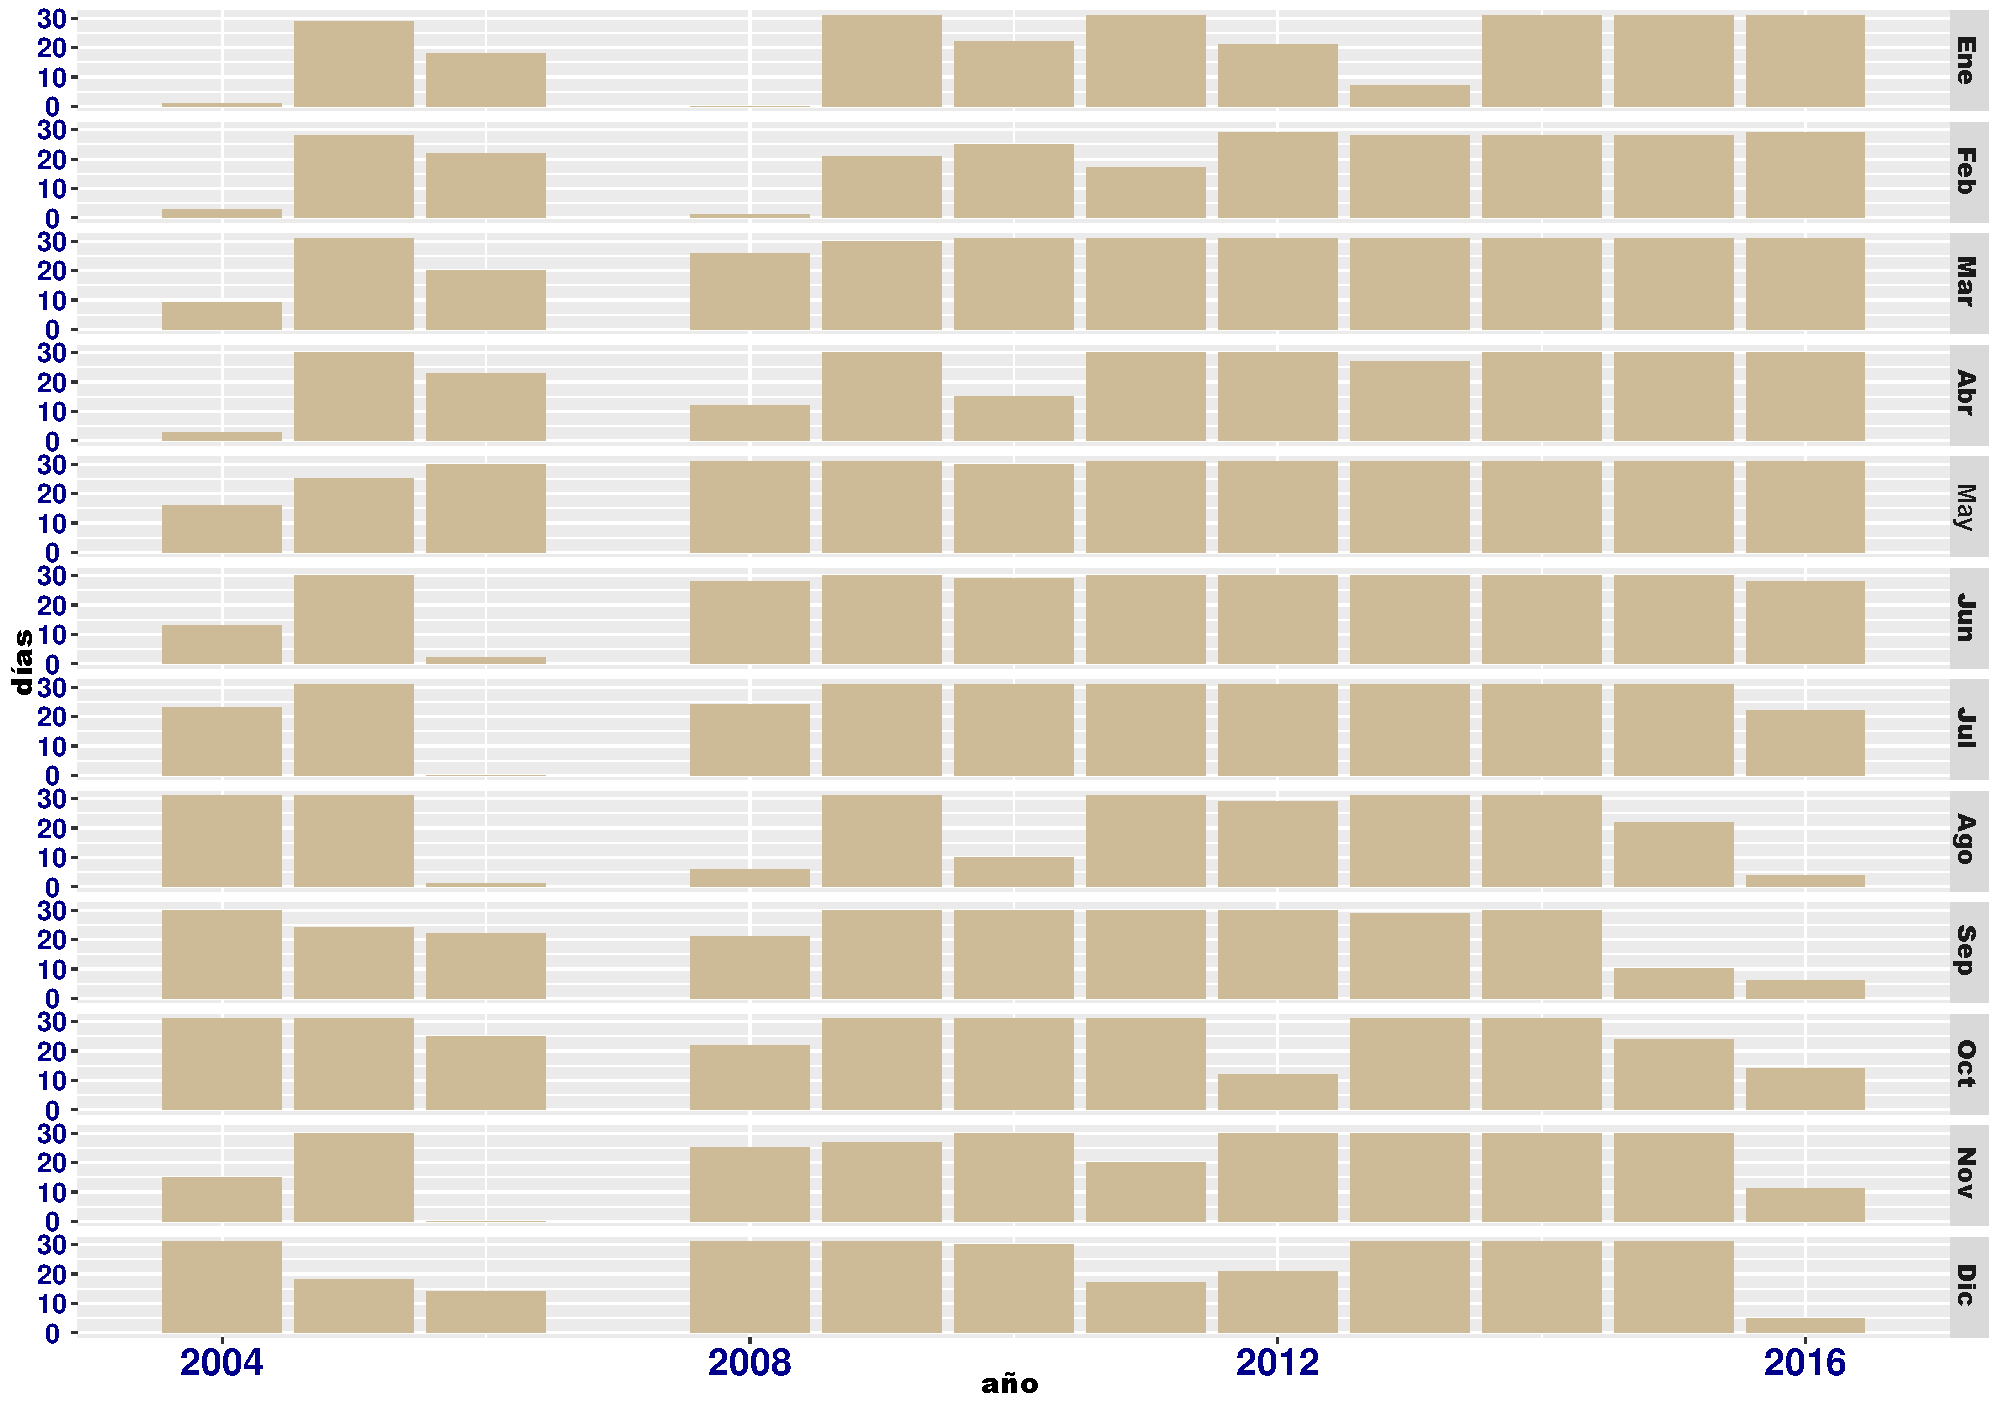
\includegraphics[scale=0.45]{Capitulo2/figs/detectados.pdf}      %Ruta completa de la imagen, porque se compila desde el archivo tesis.tex
  
  \caption{Gráfica que muestra el número de días registrados por mes y año.}            %Pie de imagen
  \label{detec}                            %nombre de referencia
\end{figure}

Es importante destacar que la gráfica sólo muestra la cantidad de días en que hubo registros, lo cual no quiere decir que todos los datos registrados sean ``buenos". Por ejemplo, en abril del 2010 hubo varios cortes de energía que duraron más de un día. Así varios archivos no tienen datos, los datos son constantes o los archivos están interrumpidos porque el soporte de energía era de 18 horas y el corte respectivo fue mayor.\\
  
También en septiembre de 2010, varios días tienen datos con ceros, debido a cortes en el suministro de energía eléctrica. Este problema persistió hasta principios de 2011. En el \emph{capítulo 3} se mostrará el porcentaje de datos confiables.\\

\section{Estructura de archivos registrados}

Antes de pasar al siguiente capítulo para mostrar los códigos usados al importar los datos, es necesario conocer cómo están estructurados. Se han manejado varias razones de conteo: de 3 segundos, 10 segundos y un minuto.\\

En la Tabla \ref{min} se muestran las primeras y últimas filas del archivo mx040720.sn1, que contiene datos del 20 de julio de 2004. La primera columna denota el año en que se está llevando a cabo el registro, en este caso 2004; la segunda columna contiene el número del mes y el día, es decir, 720 indica que es el día 20 del mes 7 (julio). En la columna 3 se encuentra el tiempo, empieza con el minuto 0, sigue el minuto 1, 2, 3 , 4 hasta llegar al minuto 59 y luego 100 que denota la hora 1 con cero minutos. Se sigue con 101,102 hasta llegar a 159, luego 200, que es la hora 2 con cero minutos. De esta manera, llega a la fila 1440 a la hora 23 con 59 minutos y termina con el minuto 0 del siguiente día.\\

La cuarta columna no es ningún dato relevante. De la columna 5 a la 8 son los datos de partículas neutras (canales S1\_A, ..., S4\_A), de la columna 9 a la 12 son datos de partículas cargadas desde S1 hasta S4. Luego siguen otras 378 columnas con registro de otros datos que no se usarán para este trabajo.\\  


\begin{table}[H]
  \centering
\centering
\begin{tabular}{r|cccccccccccc}
  & 1 & 2 & 3 & 4 & 5 & 6 & 7 & 8 & 9 & 10 & 11 & $\cdots$ \\
  \hline
1 & 2004 & 720 &   0 & 100 & 8761 & 3407 & 1196 & 541 & 27371 & 12855 & 5036 & $\cdots$\\ 
  2 & 2004 & 720 &   1 &   0 & 8602 & 3355 & 1187 & 539 & 27619 & 13003 & 5083 & $\cdots$\\ 
  3 & 2004 & 720 &   2 &   0 & 8705 & 3402 & 1261 & 580 & 27804 & 13205 & 5194 & $\cdots$\\ 
  4 & 2004 & 720 &   3 &   0 & 8662 & 3400 & 1235 & 565 & 27645 & 12987 & 5051 & $\cdots$\\ 
  5 & 2004 & 720 &   4 &   0 & 8712 & 3323 & 1178 & 551 & 27702 & 12876 & 4994 & $\cdots$\\ 
  6 & 2004 & 720 &   5 &   0 & 8642 & 3271 & 1210 & 553 & 27627 & 12857 & 5107 & $\cdots$\\ 
$\vdots$ & $\vdots$ & $\vdots$ & $\vdots$ & $\vdots$ & $\vdots$ & $\vdots$ & $\vdots$ & $\vdots$ & $\vdots$ & $\vdots$ & $\vdots$ &  \\
  1436 & 2004 & 720 & 2355 &   0 & 8577 & 3316 & 1204 & 569 & 27647 & 13057 & 5104 & $\cdots$\\ 
  1437 & 2004 & 720 & 2356 &   0 & 8652 & 3358 & 1233 & 561 & 27647 & 12928 & 5083 & $\cdots$\\ 
  1438 & 2004 & 720 & 2357 &   0 & 8665 & 3400 & 1231 & 545 & 27596 & 12999 & 5039 & $\cdots$ \\ 
  1439 & 2004 & 720 & 2358 &   0 & 8732 & 3399 & 1226 & 548 & 27675 & 12983 & 5060 & $\cdots$\\ 
  1440 & 2004 & 720 & 2359 &   0 & 8681 & 3355 & 1152 & 557 & 27789 & 12983 & 5009 & $\cdots$\\ 
  1441 & 2004 & 721 &   0 &   0 & 8651 & 3377 & 1252 & 558 & 27848 & 13032 & 5098 & $\cdots$\\ 
  
\end{tabular}

\caption{Datos del 20 de julio de 2004, razón de conteo de 1 minuto.}
\label{min}     
\end{table}


Ahora véase la Tabla \ref{10seg}, con datos del 1 de junio de 2008, esta es la estructura de los archivos registrados cada 10 segundos. Las primeras cinco filas contienen información acerca del registro de ese día, como \emph{INTERVAL} que indica el intervalo de tiempo entre cada observación, \emph{DATE}  contiene la fecha en el formato año, mes y día (080601, 1 de junio de 2008). TIME es la hora o tiempo en que empieza el registro, en este caso 000000 indica que empieza a las 0 horas, 0 minutos con 0 segundos. Mientras que la última fila ( fila 8646) dice que el archivo termina con 8640 observaciones.\\

Como se puede ver, las primeras cinco filas son innecesarias, ya que la columna 2 contiene la fecha en el mismo formato para cada observación, así como la columna 3 guarda la hora, minuto y segundo. De la columna 4 a la 7 son datos de partículas neutras (canales S1\_A, ..., S4\_A), mientras que la columna 8 a la 11 guarda datos de partículas cargadas (S1, ..., S4). En total el archivo contiene 52 columnas.\\


\begin{table}[H]
  \centering
\begin{tabular}{r|llccccccccc}
  & 1 & 2 & 3 & 4 & 5 & 6 & 7 & 8 & 9  & $\cdots$\\
\hline

 1 & NCHANNEL &         48 &        &      &     &   &    &  &  &       \\

 2 & INTERVAL &         10 &        &        &      &      &    &  & &   \\

 3 & VERSION &       3.00 &        &       &       &      &     &  & &       \\

 4 & DATE &      080601 &        &         &       &      &    &    & &      \\

 5  & TIME &      000000 &        &        &       &      &   &   & &     \\

  6 & SG & 080601 & 000010 & 12400 & 4120 & 1108 & 108 & 26692 & 11292  & $\cdots$\\ 
  7 & SG & 080601 & 000020 & 12408 & 4100 & 1036 &  12 & 26656 & 11372  & $\cdots$\\ 
  8 & SG & 080601 & 000030 & 12364 & 4124 & 1104 & 104 & 26636 & 11344  & $\cdots$\\ 
  9 & SG & 080601 & 000040 & 12292 & 4108 & 1024 & 124 & 26664 & 10292 & $\cdots$\\ 
  10 & SG & 080601 & 000050 & 12348 & 4216 & 1148 &  60 & 26632 & 11364 & $\cdots$\\ 
  11 & SG & 080601 & 000100 & 12412 & 4188 & 1028 &   0 & 26740 & 10260 & $\cdots$\\ 
  $\vdots$ & $\vdots$ & $\vdots$ & $\vdots$ & $\vdots$ & $\vdots$  & $\vdots$ & $\vdots$ & $\vdots$ & $\vdots$ &  \\
  8641 & SG & 080601 & 235920 & 12408 & 4108 & 1136 &   4 & 26704 & 10316 & $\cdots$\\ 
  8642 & SG & 080601 & 235930 & 12412 & 4096 & 1120 & 100 & 26656 & 10320 & $\cdots$\\ 
  8643 & SG & 080601 & 235940 & 12364 & 4140 & 1144 &   8 & 26732 & 11352 & $\cdots$\\ 
  8644 & SG & 080601 & 235950 & 12400 & 4128 & 1072 & 120 & 26648 & 11356 & $\cdots$\\ 
  8645 & SG & 080602 & 000000 & 12316 & 4100 & 1060 &  96 & 26740 & 10284 & $\cdots$\\ 
  8646 & END & 8640 &  &  &  &  &  &  &  & \\ 

\end{tabular} 
\caption{Datos del 1 de junio de 2008, razón de conteo 10 segundos.}
\label{10seg}       
\end{table}

Nótese en la Tabla \ref{3seg} que la estructura para archivos con razón de conteo 3 segundos es igual para los archivos con datos de registro cada 10 segundos. Lo único en que difieren es en la cantidad de filas u observaciones.


\begin{table}[H]
  \centering
\begin{tabular}{r|llccccccccc}
  & 1 & 2 & 3 & 4 & 5 & 6 & 7 & 8 & 9  & $\cdots$\\
\hline

 1 & NCHANNEL &         48 &        &      &     &   &    &  &  &      \\

 2 & INTERVAL &         2 &        &        &      &      &    &  & &   \\

 3 & VERSION &       3.00 &        &       &       &      &     &  & &       \\

 4 & DATE &      080310 &        &         &       &      &    &    & &      \\

 5  & TIME &      000000 &        &        &       &      &   &   & &       \\

  6 & SG & 080310 & 000003 & 4120 & 1104 &  88 &  80 & 7184 & 3164 &$\cdots$ \\ 
  7 & SG & 080310 & 000006 & 4172 & 1148 & 112 &  84 & 8248 & 3144 &$\cdots$\\ 
  8 & SG & 080310 & 000009 & 4192 & 1140 & 120 & 104 & 8196 & 3112 &$\cdots$\\ 
  9 & SG & 080310 & 000012 & 4148 & 1132 & 112 &  76 & 7224 & 3176 &$\cdots$\\ 
  10& SG & 080310 & 000015 & 4196 & 1104 & 108 & 116 & 8240 & 3080 &$\cdots$\\ 
  $\vdots$ & $\vdots$ & $\vdots$ & $\vdots$ & $\vdots$ & $\vdots$  & $\vdots$ & $\vdots$ & $\vdots$ & $\vdots$ &  \\ 
  28802 & SG & 080310 & 235951 & 3196 & 1060 &  12 &   0 & 7288 & 3076 &$\cdots$\\ 
  28803 & SG & 080310 & 235954 & 4124 & 1060 & 116 & 108 & 7212 & 3192 &$\cdots$\\ 
  28804 & SG & 080310 & 235957 & 4116 & 1120 &   0 & 100 & 8288 & 3096 &$\cdots$\\ 
  28805 & SG & 080311 & 000000 & 4200 & 1124 & 124 & 100 & 7256 & 3152 &$\cdots$\\ 
  28806 & END & 28800 &  &  &  &  &  &  & &  \\ 

\end{tabular} 
\caption{Datos del 10 de marzo de 2008, razón de conteo 3 segundos.}
\label{3seg}       
\end{table}

En el \emph{capítulo 3} se explica el código para realizar esta lectura de datos en R.\\
 
 
Ahora que se conoce la estructura de los datos, el objetivo es prepararlos para el posterior análisis. Para un manejo más eficiente, es necesario tener una sola columna que contenga la fecha y hora, así como una columna con el respectivo nombre de la variable para cada uno de los canales de deposición de energía. Al final se tendrá un ``data frame" de 5 columnas o variables con observaciones por año. A la primera columna se le llamará ``date", representará la fecha y hora. De la segunda a la quinta columna se les llamará S1\_A, S2\_A, S3\_A, S4\_A respectivamente para cada canal de energía.\\

Como el registro se lleva a cabo en tiempo local, hay que tener especial cuidado al convertir los datos de fechas y tiempo a clase $\mathrm{``date/time"}$  en el ambiente R (Ver Capítulo 3). Para entender el procedimiento de limpieza y ordenamiento de datos, en el capítulo 3 se habla de manera resumida la sintaxis que se maneja en R para después mostrar y explicar el código usado al procesar, ordenar y realizar el análisis de datos.

           % ~20 páginas - Poner un contexto a la tesis, hacer referencia a trabajos actuales en el tema
\def\verbarg{{\scriptsize\makebox[2ex]{\arabic{VerbboxLineNo}}}\hspace{2ex}}
\chapter{R y desarrollo de códigos}

R es un lenguaje de programación para análisis estadístico y gráfico creado por Ross Ihaka y Robert Gentleman\cite{Ihaka}, se distribuye gratuitamente bajo los términos de \emph{GNU General Public Licence}\footnote{Ver \url{http://www.gnu.org/licenses/gpl.html}} y puede verse como una implementación alternativa del lenguaje S, desarrollado en AT\&T Bell Laboratories. S está disponible como el programa S-PLUS comercializado por Insightful\footnote{Para más información ver \url{http://www.insightful.com/products/splus/default.html}}.\\

R tiene una naturaleza doble de programa y lenguaje de programación. Como entorno de programación se desarrolla mediante paquetes (\textit{packages}) o bibliotecas que complementan el lenguaje con nuevos desarrollos para distintas áreas de análisis estadístico y gráfico de datos. Algunos se encuentran en el \emph{sistema base} pero muchos otros están disponibles en el sitio de internet \emph{Comprehensive R Archive Network} (CRAN) que extienden la funcionalidad. Básicamente se trata de una ventana de trabajo (consola), se pueden iniciar distintas sesiones de trabajo que podemos guardar para retomar con posterioridad en el punto que fue dejado. Los scripts consisten en una serie de instrucciones modificadas por comandos y variables ejecutadas sobre un conjunto de datos\cite{principiantes}.\\

Los archivos necesarios para instalar R, ya sea desde las fuentes o binarios pre-compilados, se
distribuyen desde CRAN \footnote{En la web \url{https://cran.r-project.org/}} junto con las
instrucciones de instalación. R esta disponible en varias formas: el código fuente escrito principalmente en C (y algunas rutinas en Fortran), esencialmente para maquinas Unix y Linux, o como archivos binarios pre-compilados para Windows, Linux (Debian, Mandrake, RedHat, SuSe), Macintosh y Alpha Unix.\\


En resumen, R proporciona un entorno de trabajo especialmente diseñado para el
análisis estadístico de datos. Sus principales características son las siguientes:
R proporciona un lenguaje de programación propio, basado en el lenguaje S, que a su vez tiene muchos elementos del lenguaje C; sin embargo, la semántica es muy distinta a la de este último. Esto es porque R permite ejecuciones de comandos en línea (compilación y ejecución unidos en un mismo paso).\\

Como cualquier lenguaje de programación, R tiene sus ventajas y desventajas:\\

\textbf{Ventajas}

\begin{itemize}
\item R es un software libre, se refiere a la libertad
de los usuarios para ejecutar, copiar, distribuir, estudiar, cambiar y mejorar el software.

\item Es multiplataforma.
\item Es de código abierto.
\item Actualización constante.
\item R es una plataforma estadística, se trata de un lenguaje creado específicamente para la visualización y exploración de datos, así que cuenta con muchas funciones de herramienta estadística.
\item Los gráficos son de calidad.
\end{itemize}


\textbf{Desventajas}

\begin{itemize}
\item Vasta documentación, esto dificulta encontrar información específica rápidamente.
\item Los mensajes de error no son tan claros.
\item Lenguaje de programación en línea de comando, es una desventaja para los que no tienen nociones de programación, aunque ayuda a entender mejor la base de la estadística.
\end{itemize}

Debido a las ventajas y herramientas de cómputo estadístico que ofrece R para la manipulación y gráfico de datos, se escogió este software para trabajar con los 13 años de detección del TNS para los cuatro canales que registran partículas neutras. En este capítulo se describirá el método utilizado, así como los paquetes usados y códigos principales para el procesamiento y manipulación de los datos. Para entrar en contexto con el lenguaje de R se da una breve introducción a la sintaxis. 

\section{Entorno de programación R}

R es un lenguaje Orientado a Objetos, además es un lenguaje interpretado (como Java) y no compilado (como C, C++, Fortran, Pascal), lo cual significa que los comandos escritos en el teclado son ejecutados directamente sin necesidad de construir ejecutables. Todas las acciones en R se realizan con objetos que son guardados en la memoria activa del ordenador, no se usan archivos temporales\cite{principiantes}. La lectura y escritura de archivos solo se realiza para la entrada y salida de datos y resultados (gráficas, etc). Los resultados se pueden visualizar directamente en la pantalla, guardar en un objeto o escribir directamente en el disco (particularmente para gráficos). Debido a que los resultados mismos son objetos, pueden ser considerados como datos y analizarlos como tal. Archivos que contengan datos pueden ser leídos directamente desde el disco local o en un servidor remoto a través de la red\cite{principiantes}.\\


Hay diferentes tipos  o clases de datos en R:
\begin{itemize}
    \item \emph{character}: cadenas de caracteres.
    \item \emph{numeric}: números reales.
    \item \emph{integer}: números enteros.
    \item \emph{complex}: números complejos.
   \item \emph{logical}: valor lógico falso (\emph{FALSE}) o verdadero (\emph{TRUE}).\\
\end{itemize}

Casi todo en R es un objeto, como son las operaciones (aritméticas o lógicas), las funciones; que constan de una lista de argumentos que se usan para realizar ciertas acciones y regresar un resultado, entre otros. El objeto más básico que puede contener alguno de los tipos de datos anteriores es el \emph{vector}, éste puede contener cero o más elementos que deben ser de la misma clase. Una manera de crear vectores es a partir de los elementos individuales que compondrán el vector\cite{santana}. Para esto se usa la función \emph{\textbf{c()}} como se muestra en la Figura \ref{consola1}.  \\

Una característica que pueden tener los objetos son los \emph{atributos}, éstos pueden ser de diferentes tipos como: nombres, dimensiones, clase, longitud, entre otros. Por ejemplo, las \emph{matrices} son un tipo de vector especial con un atributo de dimensión que indica el número de renglones y de columnas.\\
El símbolo \textbf{$<-$} es el símbolo de asignación. Para ejecutar una expresión en la consola se presiona ``Enter".

\begin{figure}[H]
  \centering
    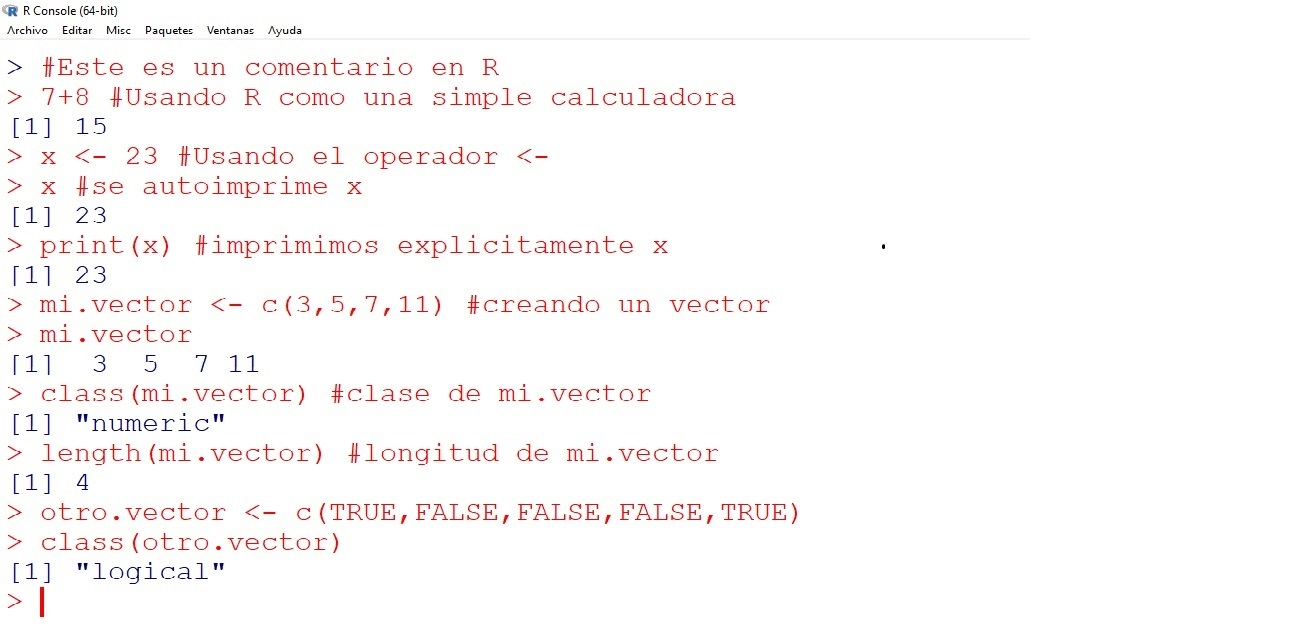
\includegraphics[scale=0.46]{Capitulo3/figs/consola1.jpg}      %Ruta completa de la imagen, porque se compila desde el archivo tesis.tex
  \caption[Entrada de datos en R]{Entrada de datos en R. El [1] que aparece a la izquierda de la salida de la expresión indica que el elemento que se encuentra a la derecha tiene índice 1.}            %Pie de imagen
  \label{consola1}                            %nombre de referencia
\end{figure}


Otros tipos de objetos son las \emph{listas} y los \emph{dataframes}. Una lista, de la clase \emph{list}, es una clase de datos que puede contener elementos de diferentes clases y de distinta longitud o dimensión. Por otro lado, un dataframe es un tipo de dato en R que sirve para guardar datos tabulares donde cada columna representa una variable, las columnas no necesariamente son de la misma clase pero deben tener la misma longitud. Para generar un dataframe se usa \emph{data.frame()}, \emph{read.table()}, \emph{read.csv()}. Ver ejemplos en la Figura \ref{consola2}.\\

\begin{figure}[H]
  \centering
    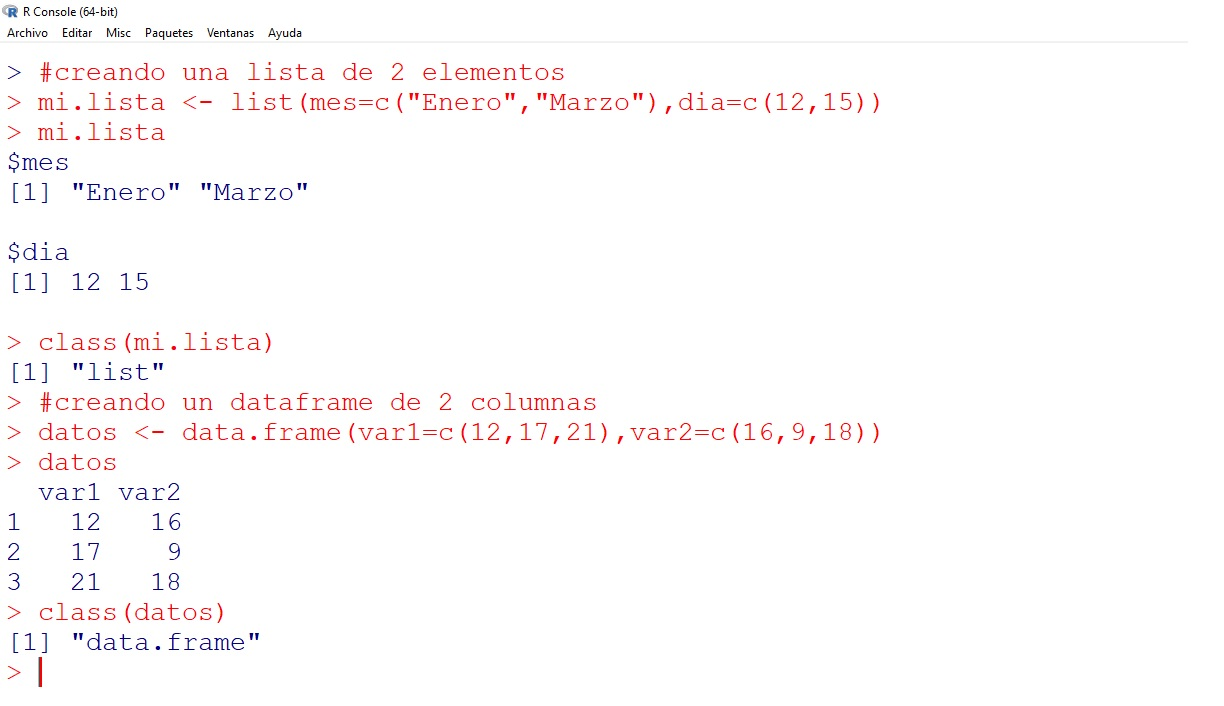
\includegraphics[scale=0.46]{Capitulo3/figs/consola2.jpg}      %Ruta completa de la imagen, porque se compila desde el archivo tesis.tex
  \caption{Creando listas y dataframes.}            %Pie de imagen
  \label{consola2}                            %nombre de referencia
\end{figure}

Para el manejo de fechas y tiempo hay clases especiales dentro del sistema. Este tipo de objetos permiten llevar a cabo operaciones numéricas y estadísticas. Hay un tipo de datos exclusivamente para fechas usando la función \emph{as.Date()}. Además, hay  2 tipos de datos para tiempo: \emph{POSIXct} y POSIXlt. La diferencia entre estos dos es la manera en que almacenan los datos internamente en R, el primero almacena el dato como el número de segundos transcurridos desde el 1 de enero de 1970, mientras que POSIXlt almacena los datos de la fecha y tiempo en forma de lista. \\

Para manipular la información de fecha y tiempo de los datos del TNS se usará la biblioteca \emph{lubridate} porque es más eficiente al hacer la conversión en grandes cantidades de datos  que el paquete base de R. Más adelante se explica detalladamente este procedimiento.\\

En el capítulo 2 se vio cuál es la estructura de los datos, el objetivo de este capítulo es mostrar y explicar a grandes rasgos el código empleado para obtener un dataframe ordenado y el método para hacer la limpieza de datos.

\section{Limpieza y ordenamiento de datos}

La limpieza de datos es una parte esencial del análisis estadístico. De hecho, en la práctica lleva aún más tiempo que el análisis en sí. La limpieza de datos o \emph{data cleaning} es el proceso de transformación de datos crudos en datos consistentes que puedan ser analizados. Si bien el orden de las variables y las observaciones no afectan al análisis, un buen orden hace que sea más fácil que un analista o una computadora extraigan las variables necesarias porque proporciona una forma estándar de estructurar un conjunto de datos.\\

De acuerdo al artículo \textit{Tidy Data} de Hadley Wickham\cite{tidy-data} los datos ordenados deben cumplir con lo siguiente:

\begin{enumerate}
\item Cada variable forma una columna.
\item Cada observación forma una fila. 
\item Cada tipo de unidad observacional forma una tabla.
\end{enumerate}

En esta sección describiré como ordené los datos del TNS de acuerdo a los principios mencionados anteriormente y extrayendo sólo las variables que nos interesan (datos que registran partículas neutras y la fecha y tiempo).\\

El lenguaje R puede leer datos guardados como archivos de texto plano, del tipo \emph{.csv}, \emph{.txt}, \emph{.dat}. También lee archivos en otros formatos (Excel, SAS, SPSS) pero las funciones necesarias no están incluidas en el paquete \emph{base}. Para leer y escribir archivos, R utiliza el directorio de trabajo. Para conocer el directorio se utiliza el comando \emph{getwd()}\footnote{get working directory}. Para cambiar el directorio de trabajo se utiliza la función \emph{setwd()} utilizando como argumento la dirección (path).\\

En el capítulo anterior se comentó que los datos del TNS se guardan en archivos con extension \emph{.sn1}, estos son archivos de texto en formato ASCII que se pueden leer con las funciones \emph{read.table()}, \emph{read.csv()}, \emph{read.csv2()}; las cuales regresan un objeto de tipo \emph{data frame}. Como no es necesario tener el conjunto completo de datos (13 años) todo el tiempo en una sesión de  R, se procesó la información por año.\\ 

Para leer y ordenar los datos del TNS se usaron dos códigos distintos, uno para los datos registrados por minuto y otro para los que se registraron cada 3 y 10 segundos. Estos últimos aún cuando no tengan la misma razón de conteo, los archivos sí tienen la misma estructura por lo que no hay necesidad de tratarlos por separado, ya que en R se pueden hacer operaciones con fechas y tiempos para ponerlos en una misma razón de conteo cuando sea necesario.\\

A continuación se explican los códigos mencionados anteriormente, el primero es un ejemplo para datos de 2005 y el segundo es para el año 2008. Para los demás años se procede de la misma forma que en alguno de los dos casos.\\

Procesamiento de datos para 2005:

Primero se cambia el directorio de trabajo a la carpeta donde se encuentran los archivos de 2005. En la línea 2 se obtienen los nombres de estos archivos y se guarda en la variable ``archivos". En la línea 3 se crea la función \emph{leer1}, ésta recibe un parámetro que se usa en la función \emph{read.table()} y solo va a leer las columnas del 1 al 3 y luego del 5 al 12. En la línea 4, con la función lapply, se aplica la función leer1 con cada una de las entradas del vector archivos, el resultado es una lista con elementos que son dataframes, se guarda en dat05. Por último, en la línea 5 se extrae cada entrada de la lista dat05 y con rbind cada dataframe se ``pega" \, uno debajo de otro. El resultado es un dataframe que contiene todos los datos de 2005 con las columnas del 1 al 3 y del 5 al 12.\\

\begin{mybox}
\begin{Verbatim}[numbers=left,xleftmargin=5mm]
> setwd("./Data_TNS/2005")
> archivos <- list.files()
> leer1 <- function(file){read.table(file)[c(1:3,5:12)]}
> dat05 <- lapply(archivos,leer1)
> dat05 <- do.call(rbind,dat05)
\end{Verbatim}
\end{mybox}

Ya se tienen los datos del año 2005 en un dataframe, falta poner en una sola columna la información de fecha y tiempo para cada observación en el formato año-mes-día hora:minuto:segundo, se hace en el \emph{Paso 2} y \emph{Paso 3}. La primera línea calcula la cantidad de ``ceros" que le falta a cada elemento de la columna 3 para que sean 4 dígitos, y devuelve esa cantidad de ceros en un vector temp. La segunda línea pega el vector temp con la columna 3 de dat05 y otros dos ceros al final, esta operación es elemento a elemento y se ``reescribe" \, en la columna 3. La tercera línea muestra las primeras 4 filas del resultado.\\

Paso 2:
\begin{mybox}
\begin{verbatim}
> temp <- mapply(function(x, y) paste0(rep(x, y), 
	collapse = ""), 0, 4 - nchar(dat05$V3))
> dat05$V3 <- paste0(temp, dat05$V3,00)
> head(dat05,4)
    V1  V2   V3     V5   V6   V7  V8    V9   V10  V11  V12
1 2005 101 000000  9147 3365 1217 561 27783 12932 5109 2476
2 2005 101 000100  9099 3458 1215 574 27809 12872 5039 2446
3 2005 101 000200  8979 3415 1200 526 27854 13016 5014 2415
4 2005 101 000300  8981 3434 1194 573 27917 13013 5079 2484
\end{verbatim}
\end{mybox}

Para el \emph{Paso 3} se instaló previamente la biblioteca \emph{dplyr} (se explica en la siguiente sección), se carga a la sesión de R en la primera línea. La segunda línea es una nueva gramática del paquete dplyr, lo primero que hace es tomar el dataframe dat05, con mutate le agrega una nueva columna llamada \emph{date} que es el resultado de pegar las columnas V1,V2 y V3. Posteriormente, con \emph{select} extrae solo las variables de interés, date y datos de los ocho canales. Luego, con \emph{rename} le pone nombres a las variables. Por último, se muestran las primeras cuatro líneas del resultado y en la última línea guarda el dataframe en una ventana de datos de R, en dat05.RData.\\

Paso 3:
\begin{mybox}
\begin{verbatim}
> library(dplyr)
> dat05 <- dat05 %>% mutate(date = paste(V1,0,V2," ",V3)) %>%
	select(date,V5:V12) %>%
	rename(S1_A=V5,S2_A=V6,S3_A=V7,S4_A=V8) %>%
	rename(S1=V9,S2=V10,S3=V11,S4=V12)
> head(dat05,4)
             date  S1_A S2_A S3_A S4_A  S1    S2   S3   S4 
1 20050101 000000  9147 3365 1217 561 27783 12932 5109 2476
2 20050101 000100  9099 3458 1215 574 27809 12872 5039 2446
3 20050101 000200  8979 3415 1200 526 27854 13016 5014 2415
4 20050101 000300  8981 3434 1194 573 27917 13013 5079 2484
> save(dat05,file="dat05.RData")
\end{verbatim}
\end{mybox}

Ahora véase el ejemplo para el año 2008, el primer paso es igual que el ejemplo anterior, solo difieren en la función \emph{leer2} porque los archivos tienen otra estructura, en este caso  se leerán las columnas del 2 al 11.\\

Ejemplo para datos de 2008.
\begin{mybox}
\begin{Verbatim}[numbers=left,xleftmargin=5mm]
> setwd("./Data_TNS/2008")
> archivos <- list.files()
> leer2 <- function(file){read.csv2(file,header=F,skip=5,sep=" ",
	colClasses=c(rep("character",3),rep("integer",49)))[2:11]}
> dat08 <- lapply(archivos,leer2)
> dat08 <- do.call(rbind,dat08)
\end{Verbatim}
\end{mybox}

El siguiente paso es similar al Paso 3 del ejemplo anterior. Se toma el dataframe dat08, con mutate se le agrega la columna date y con select se extraen las columnas date y datos de los ocho canales. Al final se guarda el dataframe en la ventana de datos \emph{dat08.RData}.\\

Paso 2:
\begin{mybox}
\begin{verbatim}
> library(dplyr)
> data08 <- dat08 %>% mutate(date = paste(V2,V3)) %>%
	select(date,V4:V11) %>%
	rename(S1_A=V4,S2_A=V5,S3_A=V6,S4_A=V7) %>%
	rename(S1=V8,S2=V9,S3=V10,S4=V11)
> save(dat08,file="dat08.RData")
\end{verbatim}
\end{mybox}

Como se ha mencionado anteriormente, hay varios paquetes que se han desarrollado para complementar el lenguaje de R. Si bien muchos paquetes desarrollan nuevos algoritmos, hay otros que realizan acciones que se pueden llevar a cabo con el paquete base. La ventaja de estas bibliotecas es que reducen el tiempo de ejecución cuando se trabaja con grandes cantidades de datos y el lenguaje es más intuitivo, por ejemplo \emph{lubridate} y \emph{dplyr}.\\ 

Hasta este punto se tienen los datos ordenados del TNS para cada año y todos tienen la misma estructura, pero falta ``decirle" \, a R que la columna \emph{date} de cada dataframe es una columna de fechas y tiempo. Para convertir esta columna en clase ``date/time" se usará la biblioteca \emph{lubridate}, el código se muestra en la siguiente sección así como una breve descripción de los paquetes que permitieron trabajar los datos del TNS de manera eficiente.\\

\section{Paquetes usados de R}
Para usar los paquetes que no están incluidos en el \emph{paquete base} es necesario instalarlos. Para ello se usa la función \emph{install.packages()} con argumento entre comillas la biblioteca que se desea instalar. Después con la función \emph{library()} se carga la biblioteca al área de trabajo.

Ejemplo:
\begin{mybox}
\begin{verbatim}
>install.packages("dplyr")
>library(dplyr)
\end{verbatim}
\end{mybox}

A continuación se describen algunos paquetes en el orden en que fueron utilizados para llevar a cabo este trabajo.\\


\subsection{dplyr}
dplyr es una nueva gramática de manipulación de datos, una herramienta rápida, flexible y consistente para trabajar con datos como objetos. Entre las funciones más importantes se encuentran \emph{mutate},\emph{select}, \emph{rename}, \emph{filter}, \emph{arrange} y \emph{$group\_by$} \cite{dply}. Estas funciones fueron muy útiles al procesar los datos, como se vio en los ejemplos anteriores, ya que reduce el tiempo de ejecución comparado con las funciones que realizan la misma acción en el paquete base. Además el lenguaje es más claro y reduce líneas de código.

\subsection{lubridate}

Lubridate es un paquete de R, creado por Garrett Grolemund y Hadley Wickham, que hace mucho más fácil el trabajo con datos de fechas y horas. Identifica el orden en que aparece el año, mes y día en los datos. Además de que facilita el trabajo con zonas horarias, por defecto lubridate pone la fecha en tiempo universal (TU). En el link se pueden ver ejemplos de las herramientas que ofrece este paquete: \url{https://cran.r-project.org/web/packages/lubridate/vignettes/lubridate.html} o bien en \textit{Dates and times made easy with lubridate} de Garrett Grolemund y Hadley Wickham\cite{lubrid}.\\

Se usará esta biblioteca  para convertir a clase POSIXct la columna \emph{date} de cada tabla de datos del TNS. Como estas tablas ya tienen la misma estructura el siguiente código funciona para todas. Lo primero que se hace es localizar los índices de los datos que se registraron en horario de verano y los que no, de acuerdo a estos índices se crea un vector que contiene  CDT (Central Daylight Time) si el dato corresponde al horario de verano y  CST (Central Standard Time) si no (esta parte se trabajó de manera interactiva localizando las fechas del cambio de horario).\\ 

En el siguiente ejemplo primero se carga la bibioteca lubridate. En la segunda línea, la función \emph{merge} junta dat05 con el dataframe que tiene por columnas TZONE y OFFSET. Si la observación tiene asignado el caracter $\mathrm{``CDT"}$, en la columna OFFSET del dataframe dat05 se le asigna $-5$ y se le asigna $-6$ si tiene $\mathrm{``CST"}$.\\

Ejemplo para \emph{dat05}
\begin{mybox}
\begin{Verbatim}[numbers=left,xleftmargin=5mm]
> library("lubridate")
> data05 <- merge(dat05, data.frame(TZONE = c("CDT", "CST"), 
 	 OFFSET = c(-5, -6)))
> data_1$DATE_UTC <- ymd_hm(data_1$date, 
	 tz = "UTC") - dhours(data_1$OFFSET)
> data_1$DATE_LOCAL <- with_tz(data_1$DATE_UTC, "America/Mexico_City")
> data_1<- data_1[order(data_1$DATE_UTC), ]
\end{Verbatim}
\end{mybox}

En la cuarta línea se convierte la columna \emph{date} a clase POSIXct pero en Tiempo Universal (UTC), por lo que se le suma la cantidad de horas que faltan, estas horas se encuentran en la columna OFFSET. En la quinta línea, con la función  \emph{with\_tz} la columna DATE\_UTC se cambia a la zona horaria de $\mathrm{``America/Mexico\_City"}$, a tiempo local, y finalmente se ordenan los datos de acuerdo a la hora.\\

Es necesario convertir las fechas y horas primero en tiempo universal y despues a tiempo local, ya que si se hace lo último directamente se producen NA's en las horas repetidas, lo cual hace que la serie sea discontinua cuando si se tiene información de esos datos.

Una vez que se tuvieron los datos ordenados se procedió con la limpieza. Esta parte se trabajó de manera interactiva, explorando cómo se distribuyen los datos y detectando los valores atípicos.\\

Se observó que al procesar la información, las variables de partículas cargadas no se eliminaron. Esto debido a que se encontraron errores en el registro, había observaciones para las cuales los datos de partículas neutras eran exactamente igual a los datos de partículas cargadas, es decir, el dato del canal S1\_A igual al S1, el S2\_A igual al S2 y así hasta el S4\_A igual al S4. Además, estos datos estaban en el rango de las variables de partículas cargadas, así que se eliminaron esos índices.\\

Los ceros y datos que se repetían durante varios minutos en todos los canales se sustituyeron por NA (Not Available), que es la forma en que se denotan los valores faltantes en R, ya que era evidente que se trataba de errores electrónicos.\\

También era fácil ver que se trataba de errores aquellos datos que incrementaban y disminuían repentinamente hasta un 20\% con respecto al dato anterior y posterior. Al hablar de estabilidad de datos, lo que se busca es que la variación sea pequeña. En caso de encontrar alguna variación significativa investigar qué pudo haber afectado la toma de datos. Cuando ya no eran tan evidentes los errores se tenía que graficar la serie para ver si había variaciones importantes. Para esto, fue de mucha utilidad el siguiente paquete.

\subsection{Openair}

La biblioteca Openair está diseñada para hacer análisis de datos de calidad del aire, sin embargo ofrece herramientas muy utiles para hacer análisis de variación en series de tiempo, sobretodo la función para agregar datos en distintos intervalos de tiempo. Es por ello que se escogió este paquete para trabajar los datos del TNS. Se puede ver más acerca del paquete en \emph{openair --- An R package for air quality data analysis}\cite{openair} y en \emph{Lenguaje R aplicado al análisis de Calidad de Aire}\cite{manualOp}.\\

Para hacer las gráficas de variación del capítulo 4 se creó la función \emph{variacion} que recibe dos argumentos, el primero es el dataframe y el segundo es el canal que se desea graficar. Luego estos parámetros se usan en la función timeVariation de openair.

\begin{mybox}
\begin{verbatim}
> library("openair")
> variacion <- function(datos,canal){
	timeVariation(datos, pollutant=canal,
	main="Variación temporal del flujo de partículas neutras",
	xlab=c("Flujo horario durante la semana","Flujo horario",
	"Flujo mensual","Variación por días de la semana"))
	}
\end{verbatim}
\end{mybox}

Así, para hacer una gráfica de variación de los datos de 2005 del canal S1\_A se hace de la siguiente forma.
\begin{mybox}
\begin{verbatim}
> variacion("dat05","S1\_A")
\end{verbatim}
\end{mybox}

Hasta este punto se ha cumplido el objetivo de tener datos ordenados y que la fecha y hora de éstos sea  reconocida como tal en R, además se limpiaron los datos de partículas neutras que eran igual a los datos de partículas cargadas. Luego se extrajeron solo la columna date y datos de los cuatro canales de interés.  A partir de aquí se empezaron a localizar los valores atípicos y ver si se debían a errores electrónicos. Sin embargo, había casos en los que el intervalo de errores era demasiado grande y por eso los datos ``correctos" eran los que se mostraban fuera de rango. Como en el caso de los datos de 2008, hasta que se graficaron los datos se observó su comportamiento. Véase el siguiente capítulo para ver las gráficas de variación por año. 



   % ~20 páginas - Explicar el problema en específico que se va a resolver, la metodología y experimentos/métodos utilizados

\chapter{Análisis de estabilidad}
\section{Introducción}

   % ~20 páginas - Presentar los resultados tal cual son, y analizarlos.
\chapter*{Conclusiones}
\addcontentsline{toc}{chapter}{Conclusiones}
\markboth{CONCLUSIONES}{CONCLUSIONES}

En este trabajo, se realizó un análisis de estabilidad estadística de las partículas neutras registradas del 2004 al 2016, por  el Telescopio de Neutrones Solares instalado en Sierra Negra, Puebla. Uno de los resultados inmediatos es que se obtuvieron datos limpios, es decir, datos sin influencia de las distintas fuentes que generan errores. Esto ayudará a saber qué datos descartar y en que intervalo de tiempo se requiere hacer un análisis más detallado si se requiere extraer información física de los mismos y estudios de física solar. Además, al usar software libre (R), nos da libertad de examinar el código, de usarlo sin restricciones, de distribuirlo y modificarlo a nuestra conveniencia; de este modo, cualquiera puede acceder y entender el código utilizado para llevar a cabo el presente trabajo, de esta manera se pueden reproducir los resultados obtenidos y mejorar y adaptar los códigos a análisis estadísticos de datos que se requieran en el futuro, ahorrando tiempo en programación.\\

Con base en las medidas de centralización y dispersión que se obtuvieron por año, se pudo observar que el $50\%$ de los datos resgistrados y confiables se encuentran cerca de la media. Por otra parte, el $25\%$ de los  datos se encuentran cerca del máximo de la variación diurna y el otro 75\% más alejado . También, analizando el coeficiente de variación se pudo observar que en la mayoría de los años (excepto 2005 y 2009)  la dispersión  de los datos que corresponden a los canales S2\_A y S3\_A fue menor comparado con los otro canales, presentando una variación menor al $8\%$. Además,  los datos del canal S4\_A se dispersan más comparado con los datos de los otros canales de energía, ya que este canal detecta partículas con mayor energía; por lo tanto, las cuentas registradas son más bajas.\\

También se ha obtenido el comportamiento de la variación diurna desde el año 2004, lo cual nos da una visión de cómo se ha llevado a cabo el registro de datos a lo largo de estos años. Además, se conoce el porcentaje anual de datos  confiables, respecto al cual se concluye que el TNS funciona de forma adecuada y que, con base en la dificultad de mantener un detector a 4580 m s.n.m., el porcentaje de datos estables es muy alta. Se conocen los intervalos temporales donde los datos no son estables y/o se tiene que hacer un análisis más detallado y particular para extraer información relevante. También conocemos las variaciones por canal de energía y podemos detectar que canal tiene problemas de software, hardware o de sistema de adquisición de datos.\\

Se concluye también que la variación diurna y señal del TNS es estable. Los errores detectados en los canales se pueden atribuir a diferentes fenómenos, como son errores en la electrónica, variaciones de voltaje, fallas en el suministro de energía eléctrica y errores de programación, que pueden generar picos y/o caídas en la toma de datos y ceros.\\

Finalmente, se observó que el programa de adquisición de datos es susceptible al hardware, ya que el cambio del servidor de adquisición y almacenaje de los datos genera errores de fecha y hora, retrasos en el tiempo de 1 a varios segundos.\\

El presente análisis concluye que el TNS en Sierra Negra funciona de forma estable y los datos registrados pueden ser usados para análisis y estudios de física solar.

            % ~5 páginas - Resumir lo que se hizo y lo que no y comentar trabajos futuros sobre el tema

%%%%%%%%%%%%%%%%%%%%%%%%%%%%%%%%%%%%%%%%%%%%%%%%%%%%%
%                   APÉNDICES                       %
%%%%%%%%%%%%%%%%%%%%%%%%%%%%%%%%%%%%%%%%%%%%%%%%%%%%%
\appendix
% this file is called up by thesis.tex
% content in this file will be fed into the main document
\chapter{Fulguraciones solares}
% top level followed by section, subsection

Las fulguraciones solares (o llamaradas) son explosiones intensas en el Sol que viene de la liberación de la energía magnética asociada con las manchas solares. La radiación nociva de una llamarada no puede pasar a través de la atmósfera de la Tierra para afectar físicamente a los seres humanos a nivel de tierra. Aunque, cuando es suficientemente intensa,  puede afectar la ionosfera de la Tierra e interferir con nuestros sistemas de comunicaciones, como la radio y el GPS, y también perturbar la electrónica de satélites.\\


Debido la intensidad de emisión en rayos X, las fulguraciones solares se clasifican en A, B, C, M y X. Cada letra representa un aumento de 10 veces en la producción de energía\cite{nasa}. Así que una X es diez veces una M y 100 veces una C. En las figuras \ref{classM} y \ref{classX} se muestran dos clases de fulguraciones solares.\\

\begin{figure}[H]
\begin{minipage}{0.6\textwidth}
\begin{center}
\includegraphics[scale=0.05]{Apendice1/figs/claseM.jpg}
\footnote{\url{https://www.nasa.gov/content/goddard/nasa-releases-images-of-1st-notable-solar-flare-of-2015}} 
\end{center}
\end{minipage}
\hspace{0.1cm}
\begin{minipage}{0.4\textwidth}
\caption[Fulguración solar de clase M, 12 de enero de 2015]{El Sol emitió una fulguración solar de clase M, alcanzando su punto máximo a las 11:24 p.m. el 12 de enero de 2015. El Observatorio de Dinámica Solar de la NASA, que observa el sol constantemente, capturó una imagen del evento.}
\label{classM}
\end{minipage}
\end{figure}

Se recomienda ver las fotos y animaciones de las fulguraciones solares en la pestaña de galerías que se encuentra accediendo al enlace de cada imagen.

\begin{figure}[H]
  \centering
    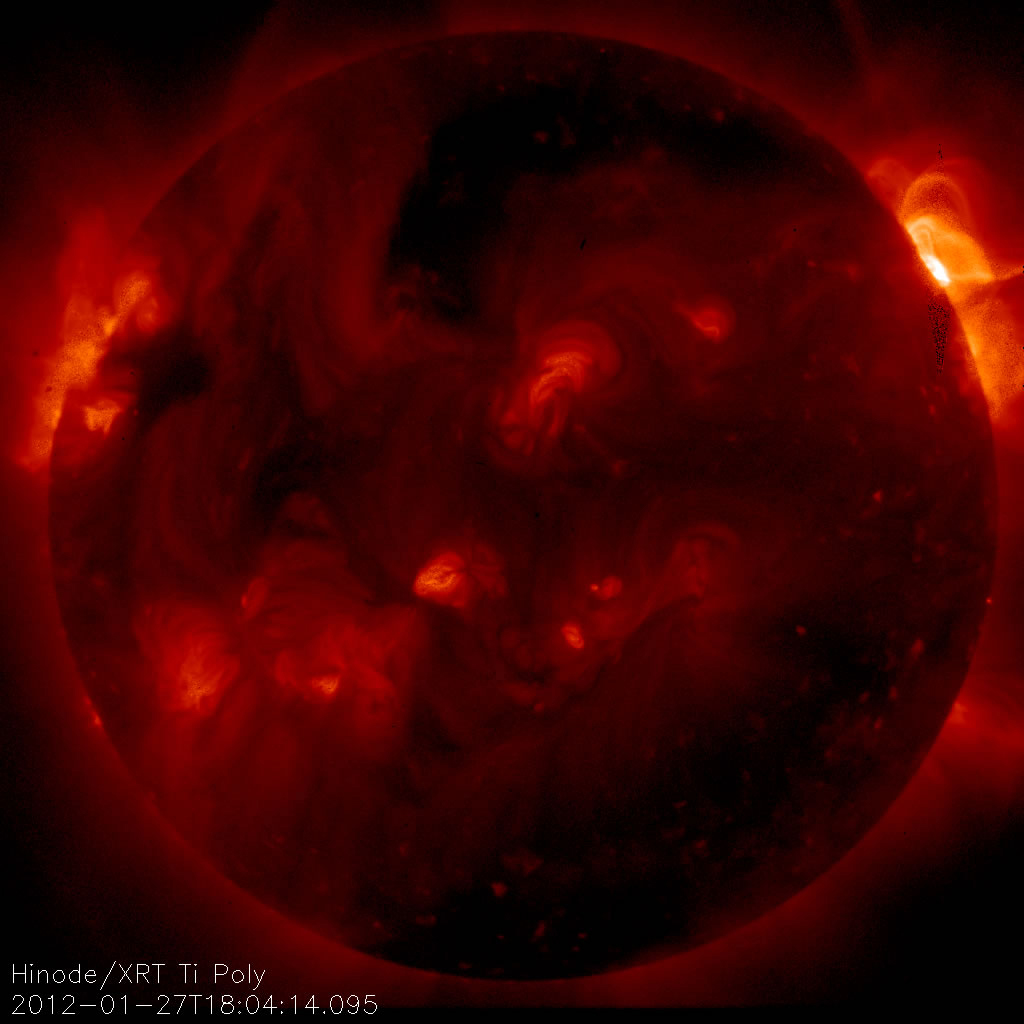
\includegraphics[scale=0.3]{Apendice1/figs/claseX.jpg}      %Ruta completa de la imagen, porque se compila desde el archivo tesis.tex
  \caption[Fulguración solar de clase X, 27 de enero de 2012]{El 27 de enero de 2012, estalló una fulguración intensa de clase X. Las fulguraciones de clase X son las explosiones más intensas. Aquí se ve una imagen de la llamarada capturada por el telescopio de rayos X en Hinode. Esta imagen muestra una emisión de plasma calentado a más de ocho millones de grados durante el proceso de liberación de energía de la llamarada. Imagen tomada de \url{https://www.nasa.gov/multimedia/imagegallery/image_feature_2169.html}}            %Pie de imagen
  \label{classX}                            %nombre de referencia
\end{figure}


\begin{figure}[H]
  \centering
    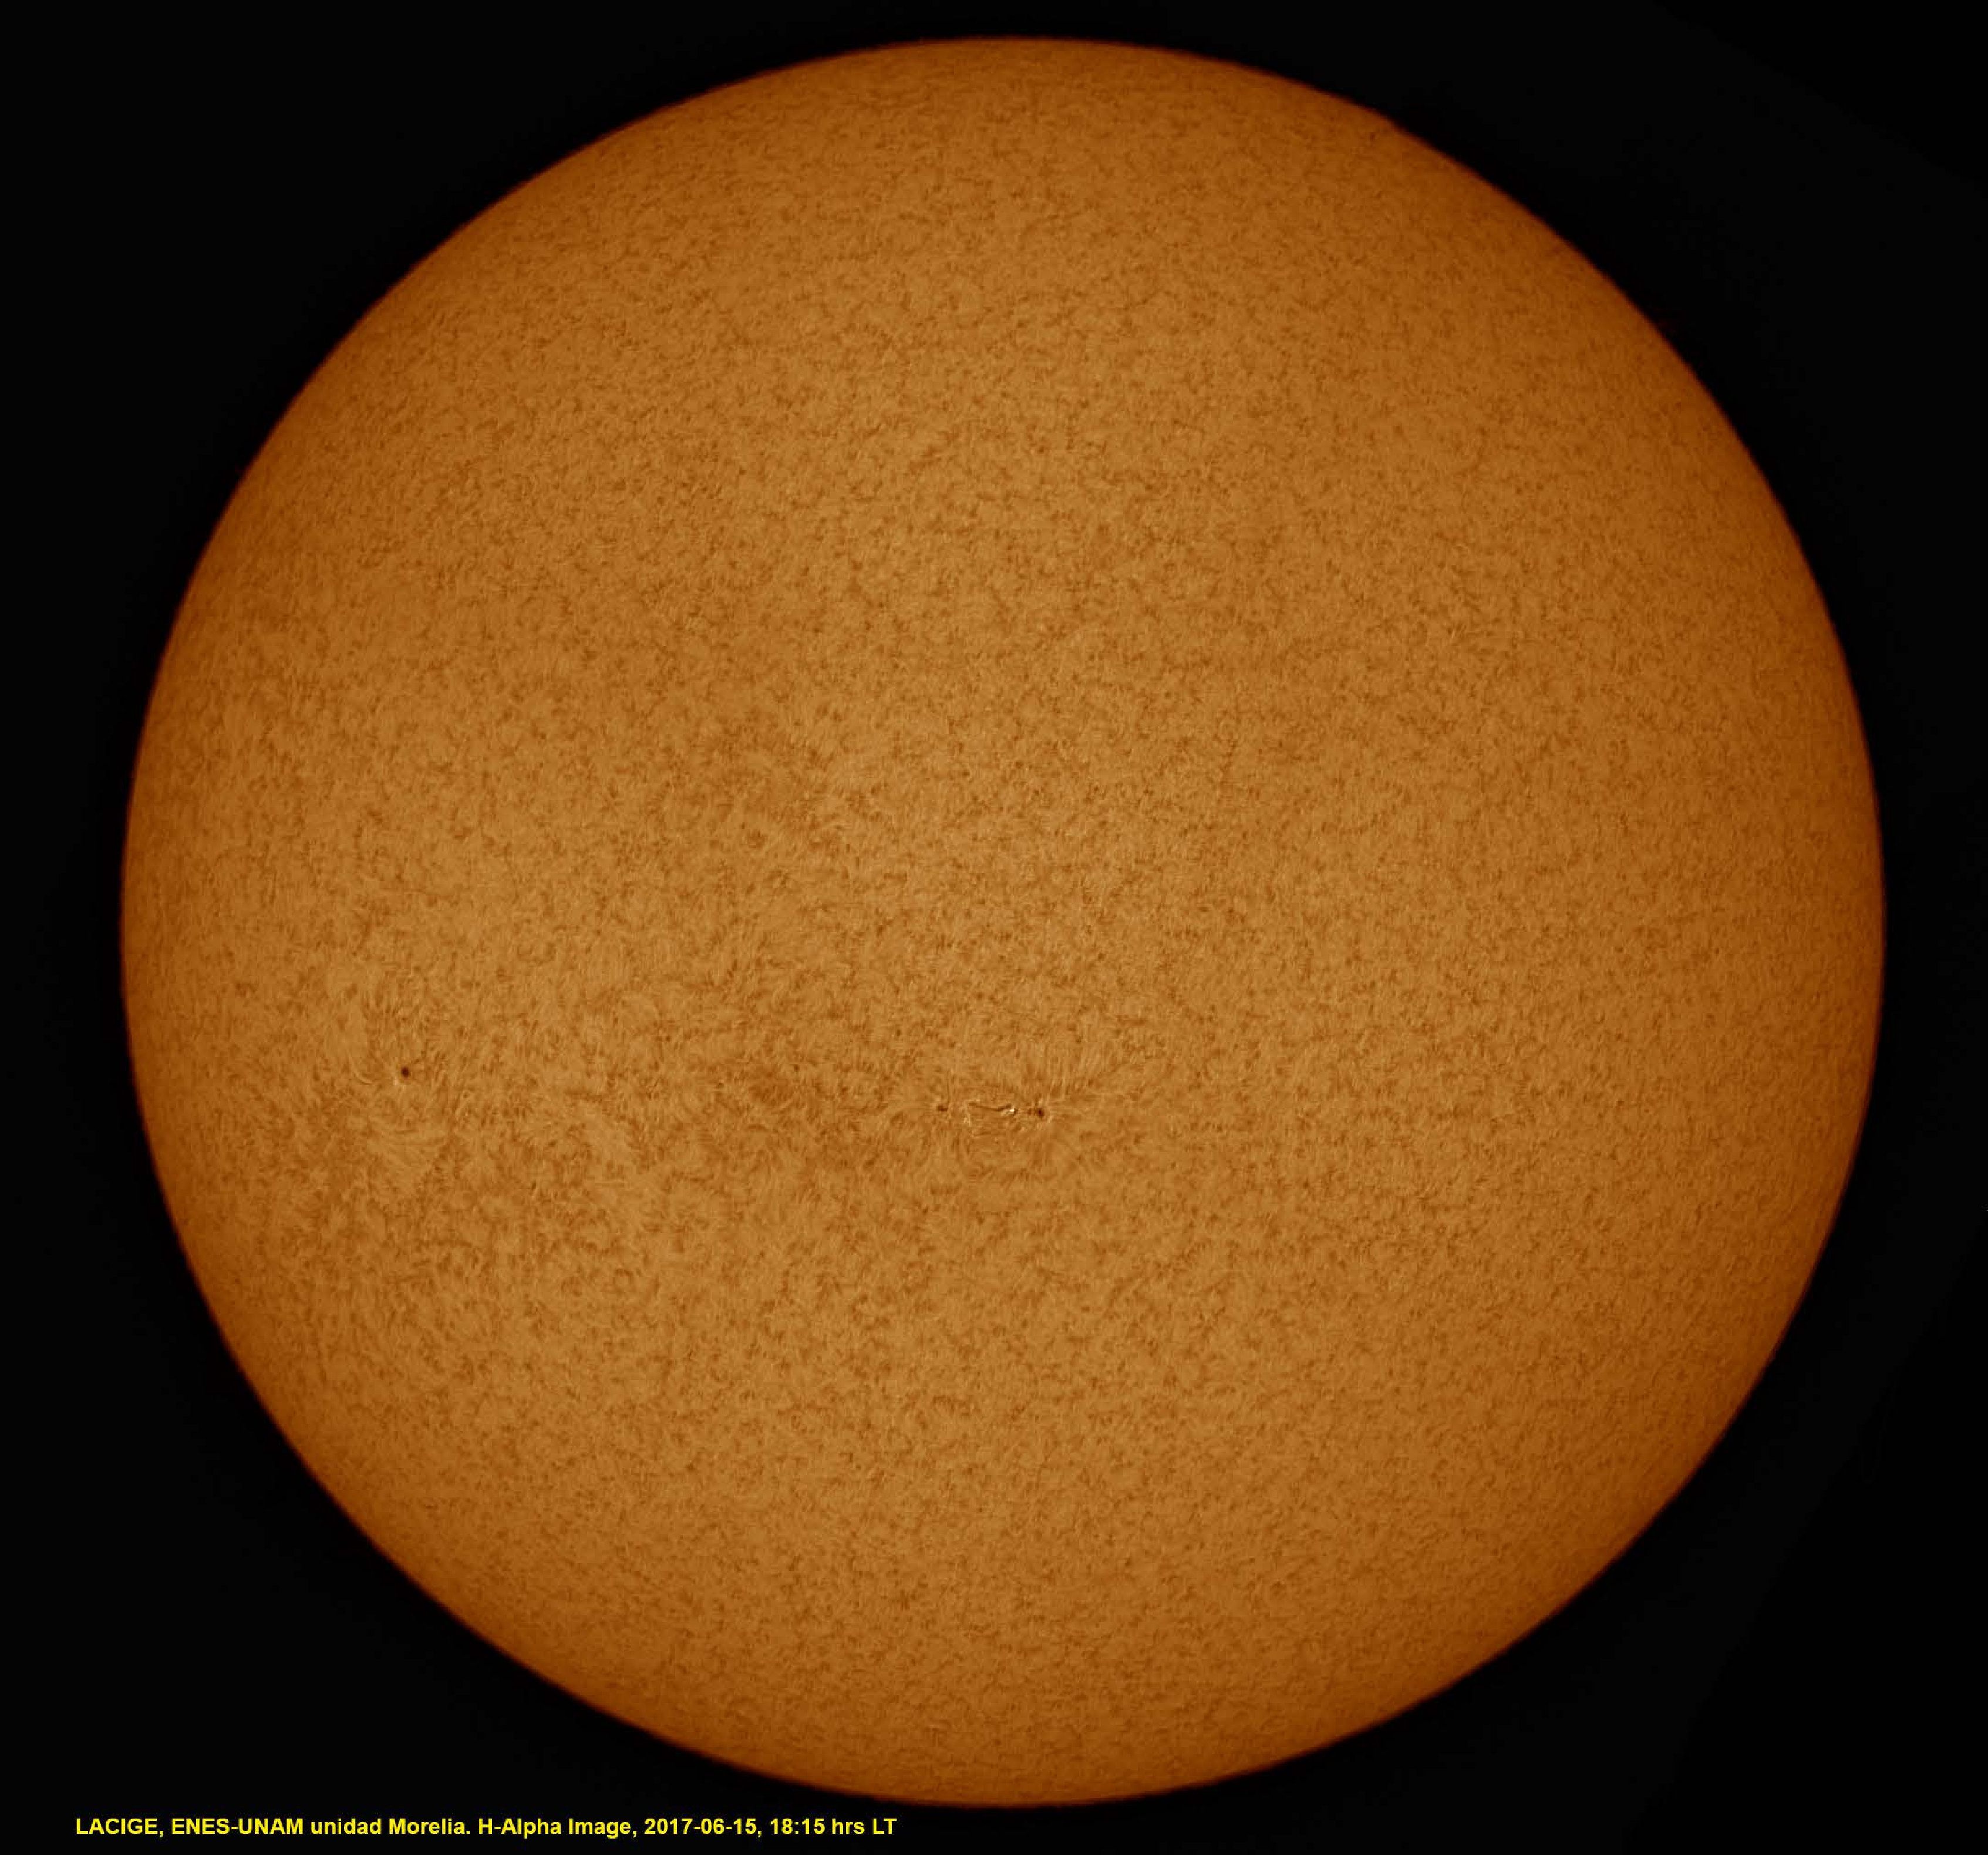
\includegraphics[scale=0.2]{Apendice1/figs/sol_compuesta.pdf}      %Ruta completa de la imagen, porque se compila desde el archivo tesis.tex
  \caption[El Sol con baja actividad]{Se muestra la imagen del Sol en el mínimo de actividad, nótese las diferencias con las figuras \ref{classM} y \ref{classX}. Es una imagen en el óptico (H-Alfa), que muestra la fotósfera solar, tomada por LACIGE, ENES-UNAM unidad Morelia.}            %Pie de imagen
  \label{minima_act}                            %nombre de referencia
\end{figure}


               % Colocar los circuitos, manuales, código fuente, pruebas de teoremas, etc.


%%%%%%%%%%%%%%%%%%%%%%%%%%%%%%%%%%%%%%%%%%%%%%%%%%%%%
%                   REFERENCIAS                     %
%%%%%%%%%%%%%%%%%%%%%%%%%%%%%%%%%%%%%%%%%%%%%%%%%%%%%
\nocite{ggmap}
\bibliographystyle{Latex/Classes/acm-es} % otros estilos pueden ser abbrv, acm, alpha, apalike, ieeetr, plain, siam, unsrt
\bibliography{Bibliografia/Bibliog}             % Archivo .bib
% existen varios estilos de bilbiografía, pueden cambiarlos a placer


%El formato trae otros estilos, o pueden agregar uno que les guste:
%\bibliographystyle{Latex/Classes/PhDbiblio-case} % title forced lower case
%\bibliographystyle{Latex/Classes/PhDbiblio-bold} % title as in bibtex but bold
%\bibliographystyle{Latex/Classes/PhDbiblio-url} % bold + www link if provided
%\bibliographystyle{Latex/Classes/jmb} % calls style file jmb.bst

\end{document}
